\section{Diseño de la Plataforma} \label{diseño}
\AddToShipoutPictureBG*{
\includegraphics[width=\paperwidth,height=\paperheight]{Imagenes/Fondo Capitulo 3.pdf}}
\thispagestyle{plain}

\vspace{0.5cm}

\Large\scshape
\begin{center}
    \textrm{Diseño de los circuitos principales y auxiliares de la plataforma}
\end{center}
\normalfont
%\normalsize

\divider

Si bien con el análisis del anterior capítulo se pudo conseguir un panorama general del funcionamiento de la plataforma, se presentan otras complejidades a la hora de plasmarlo en un sistema real: se requieren múltiples circuitos auxiliares además de los bloques principales (por ejemplo circuitos de adquisición de señales); aparecen consideraciones de diseño que no existen en el plano teórico; entre otras cuestiones. Este capítulo está dedicado al diseño real de la plataforma completa para luego implementar en una placa de circuito impreso o PCB, teniendo en cuenta estas complicaciones.\\

En la siguiente figura se muestra un diagrama detallado de la plataforma, dónde se presentan todos los distintos bloques funcionales, incluyendo los bloques auxiliares que no se trataron en el análisis del anterior capítulo.\\

\begin{figure}[h]
    \centering
    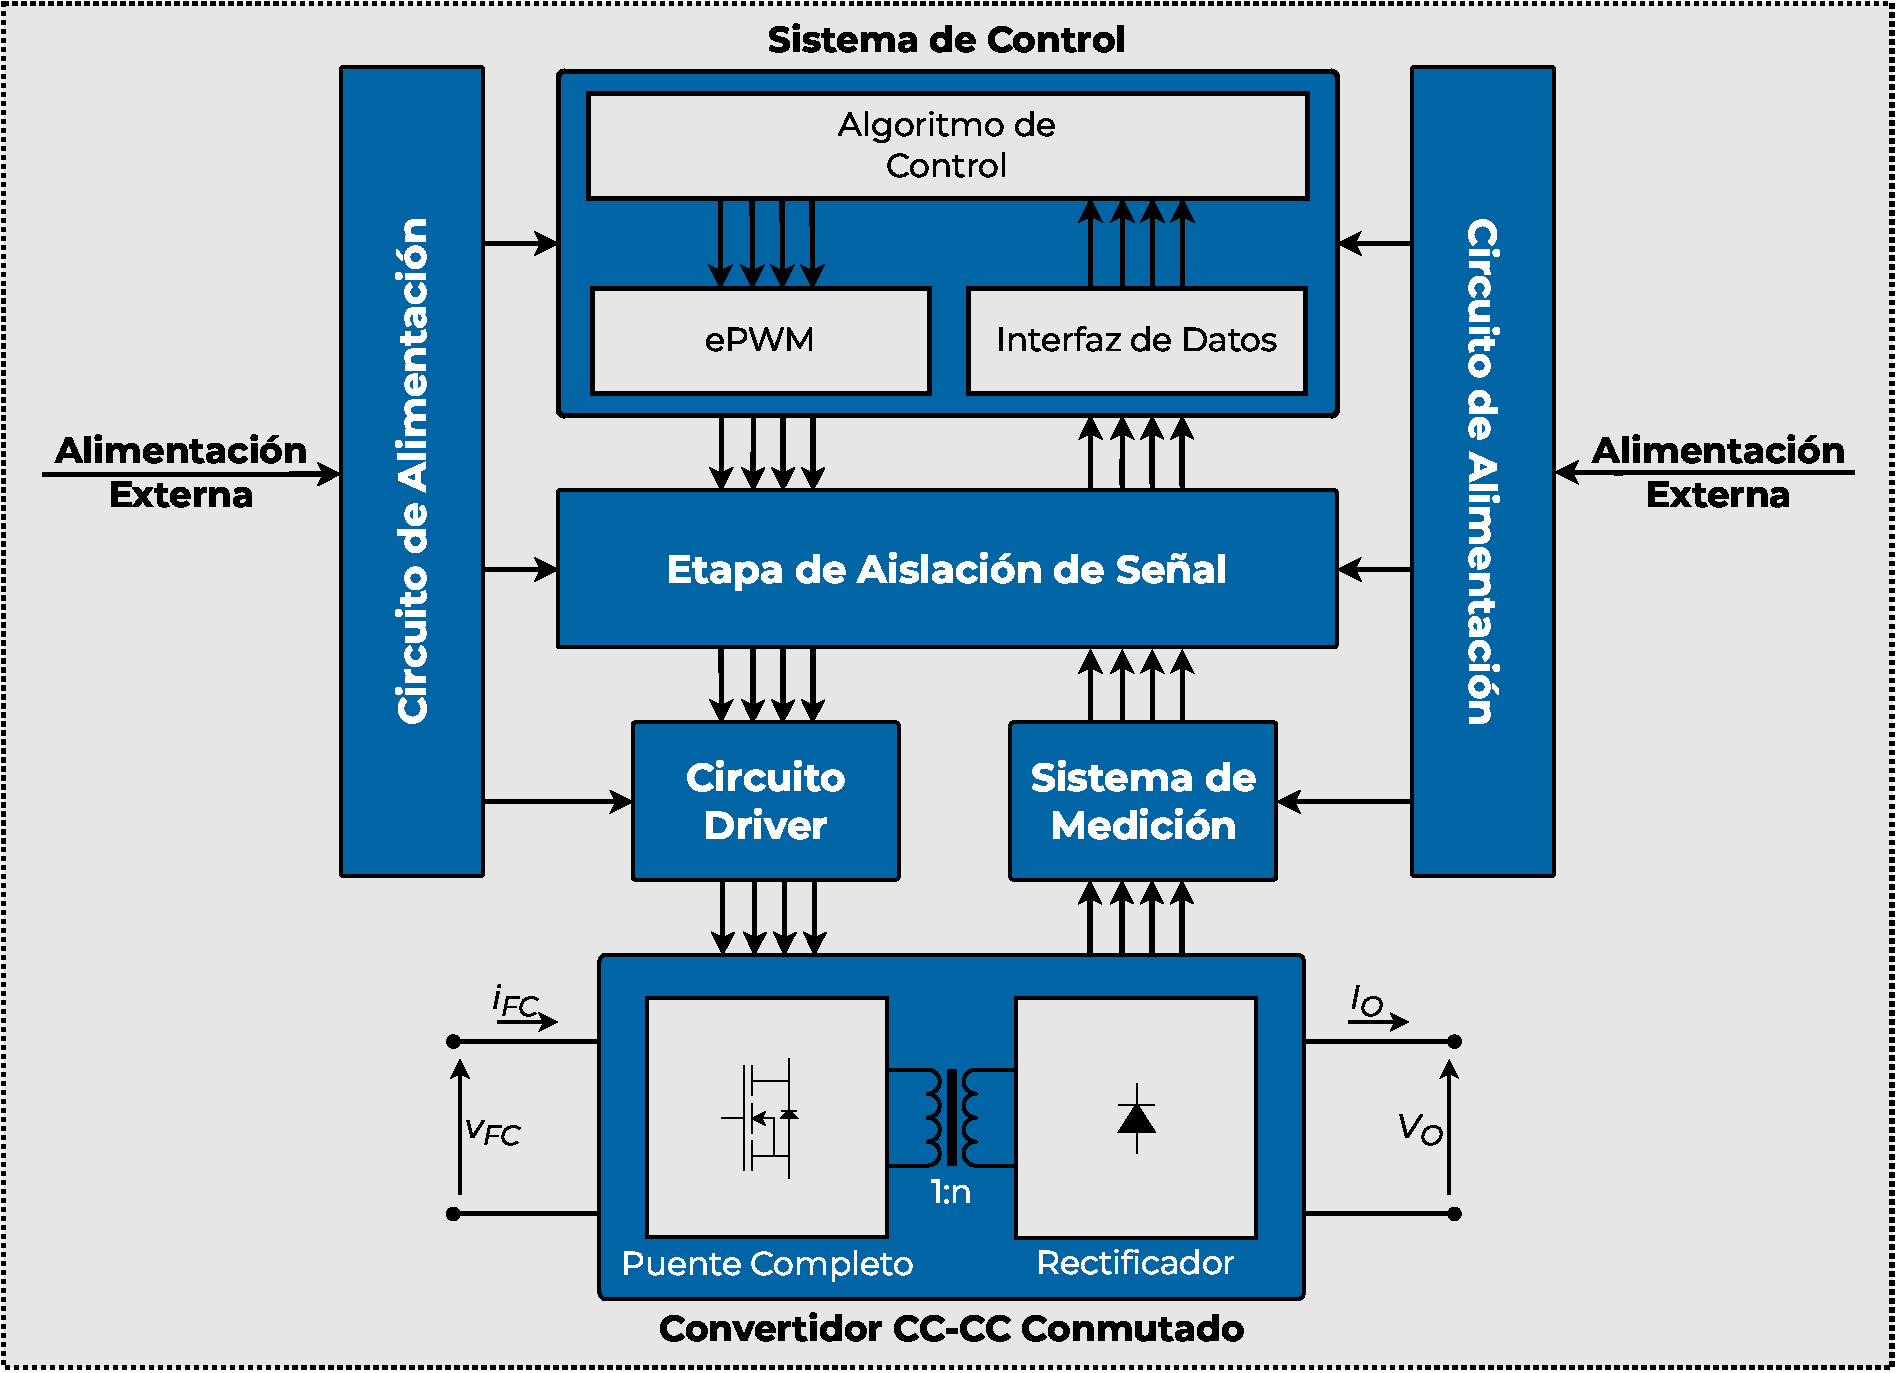
\includegraphics[scale=0.43]{Imagenes/Plataforma Detallada.pdf}
    \caption{Diagrama detallado de la plataforma de evaluación, incluyendo los distintos circuitos auxiliares.}
    \label{diag_detallado}
\end{figure}

Cada uno de estos seis bloques cumplen una función específica que se detalla a continuación:\\

\begin{itemize}
    \item {\SemiBold Convertidor CC-CC Conmutado:} Este es el convertidor de tipo puente completo que se trató en el capítulo anterior. En este capítulo se va a realizar el dimensionamiento de todos sus componentes teniendo en cuenta sus especificaciones. 
    \item {\SemiBold Circuito \textit{Driver}:} Este circuito se encarga de entregar la corriente y tensión necesaria para disparar los transistores de potencia y conmutarlos correctamente.
    \item {\SemiBold Sistema de Medición:} Este bloque contiene todos los circuitos y componentes necesarios para realizar las mediciones de todos los parámetros de interés de la plataforma. Esto incluye, además de sensores, los circuitos de acondicionamiento de señal donde se requieran.
    \item {\SemiBold Etapa de Aislación de Señal:} Esta etapa se encarga de generar una barrera de aislación eléctrica entre los componentes de potencia y los componentes de señal del circuito.
    \item {\SemiBold Sistema de Control:} Este es el bloque de control que se explicó en el anterior capítulo. Obtiene información de distintos parámetros por medio del sistema de medición, y ejerce la acción de control disparando las llaves mediante el driver.
    \item {\SemiBold Circuito de Alimentación:} Es el circuito que se encarga de proveer las corrientes y tensiones necesarias para los componentes que requieren alguna alimentación externa para funcionar (por ejemplo el controlador digital de señales).\\
\end{itemize}

A lo largo de este capítulo se va a tratar uno por uno el diseño de los circuitos que componen a cada uno de los bloques, utilizando múltiples diseños como referencia (ya sean de otros trabajos de investigación o diseños sugeridos de los propios fabricantes). Se van a eligir y dimensionanar los componentes que forman parte de ellos, hasta obtener un esquemático circuital detallado de la plataforma experimental de evaluación completa.\\

Pero antes de comenzar con el primer bloque, se van a plantear algunas consideraciones y criterios generales que se van a utilizar para la selección de todos los componentes y diseño de todos circuitos de la plataforma.\\

\subsection{Consideraciones Generales}

\subsubsection{Aislación de Tierras}

En toda la plataforma se va a trabajar con tres puestas a tierra distintas y aisladas entre sí: $GND_1$ es la tierra del primario del convertidor, $GND_2$ es la tierra del secundario del convertidor, y $GND_D$ es la tierra de las partes de señal y digitales, como los sensores y el DSC.\\

Esto, si bien agrega una mayor complejidad al diseño, es ventajoso por múltiples razones. Primero, evita la generación de interferencia de modo común entre las tierras del convertidor ($GND_1$ y $GND_2$) que manejan altas corrientes y por lo tanto son más ruidosas; y la tierra de señal $GND_D$ de más bajas corrientes que es más sensible al ruido. Además, dadas las altas corrientes del convertidor, esta separación permite la protección de los circuitos de señal ante picos de corriente y tensión inesperados en la parte de potencia.\\

Es por estas razones que además de la tierra, también los circuitos de señal y potencia se encuentran separados por la etapa de aislación entre potencia y señal. Adicionalmente, las fuentes de alimentación externas se encuentran separadas para los componentes de potencia y señal, manteniendo la aislación deseada.\\

\subsubsection{Selección de Componentes}

En líneas generales, a la hora de elegir un circuito para el diseño de los distintos bloques, si es posible se trata de elegir una solución más integrada (es decir utilizar un circuito integrado que haga esta tarea en vez de diseñar un circuito discreto). Esto simplifica los circuitos y disminuye la cantidad de componentes necesarios a la hora de implementarlos. Además, al estar toda la solución integrada, el rendimiento es más predecible y se encuentra acotado a los parámetros dados por el fabricante del circuito integrado.\\

En todos los casos, se utilizan como guía para el diseño de todas las partes los parámetros de rendimiento y las recomendaciones de diseño especificadas en las hojas de datos  y notas de aplicación de los fabricantes de cada circuito integrado.\\

\subsubsection{Herramientas de Software}

\paragraph{Software EDA}

Para realizar el diseño de todos los esquemas circuitales del sistema, y luego plasmarlos a una placa de circuito impreso se debe utilizar un herramienta de automatización de diseño electrónico o EDA (del inglés \textit{Electronic Design Automation}). Existe una gran variedad de programas que cumplen este propósito, estando entre los más conocidos el \textit{Altium Designer} de \textit{Altium}, el \textit{EAGLE} de \textit{Autodesk}, el \textit{KiCad} y el \textit{Proteus Design Suite} de \textit{Labcenter Electronics}.\\

Para este proyecto se eligió utilizar la plataforma {\Medium KiCad} (que se encuentra en la versión 6.0.7 al momento de escribir este informe), una suite de software libre, gratuita y de código abierto que incluye todas la funcionalidades necesarias para el diseño electrónico. Cuenta con herramientas de captura de esquemático, diseño de PCB, simulación mediante SPICE o Ngspice, visualización de archivos de fabricación y cálculos de diseño de PCB.\\

\begin{figure}[h]
    \centering
    
\includegraphics[scale=0.6]{Imagenes/KiCad.pdf}
    \caption{Logotipo de la plataforma KiCad EDA.}
    \label{logo_kicad}
\end{figure}

El programa también cuenta con una extensa biblioteca de componentes y \textit{footprints} (son las \quotes{huellas} de los componentes en en el circuito impreso) y la capacidad de crear o importar bilbiotecas. Además tiene la capacidad de generar archivos de fabricación, modelos tridimensionales de la PCB y una \textit{bill of materials} (lista de componentes).\\

\paragraph{Software de Simulación}

Para todo lo que se refiere a la simualción de la plataforma; más particularmente las simulaciones del funcionamiento del convertidor CC-CC para su comprensión, estudio, diseño y dimensionamiento; se utilizó la herramienta {\Medium\textit{Simulink}} dentro de la suite de software de \textit{MATLAB-Simulink}.\\

\begin{figure}[h]
    \centering
    
\includegraphics[scale=0.08]{Imagenes/Simulink.png}
    \caption{Logotipo de la plataforma de simulación Simulink.}
    \label{logo_simulink}
\end{figure}

Específicamente, para simulaciones circuitales se hizo uso de el paquete \textit{Simscape Electrical} dentro de Simulink, que permite trabajar con tensiones y corrientes, a diferencia de las herramientas estándar que trabajan con diagramas de bloques.\\

\paragraph{Otras Herramientas}

Adicionalmente, para llevar un control de versiones completo del diseño de la plataforma sobre el que se trabaja, además de mantener un historial completo de todos los cambios, se trabajó con la herramienta de software de control de versiones {\Medium\textit{Git}}.\\

\begin{figure}[h]
    \centering
    
\includegraphics[scale=0.6]{Imagenes/Git.pdf}
    \caption{Logotipo del software de control de versiones Git.}
    \label{logo_git}
\end{figure}

Con este software se crea un \textit{repositorio} donde se almacenan los archivos que se quiere controlar, manteniendo un control de la historia de cada uno de los archivos del repositorio. Para mantener los archivos sincronizados entre varias computadoras y mantener copias de seguridad, se utiliza adicionalmente la plataforma web {\Medium\textit{GitHub}} para hostear el repositorio en la nube, manteniendo una copia segura que se puede copiar a cualquier computadora.\\

\newpage

\subsection{Convertidor CC-CC Conmutado}

Para llevar a cabo el diseño del convertidor, primero debemos establecer los objetivos de rendimiento del mismo (como por ejemplo, la tensión que debe tener a la salida). Con estos valores establecidos, y junto con otras consideraciones del diseño, se van a obtener todos los parámetros que definen al convertidor, como las llaves y diodos a utilizar, tamaño de capacitores e inductores, etc.\\

\begin{figure}[h]
    \centering
    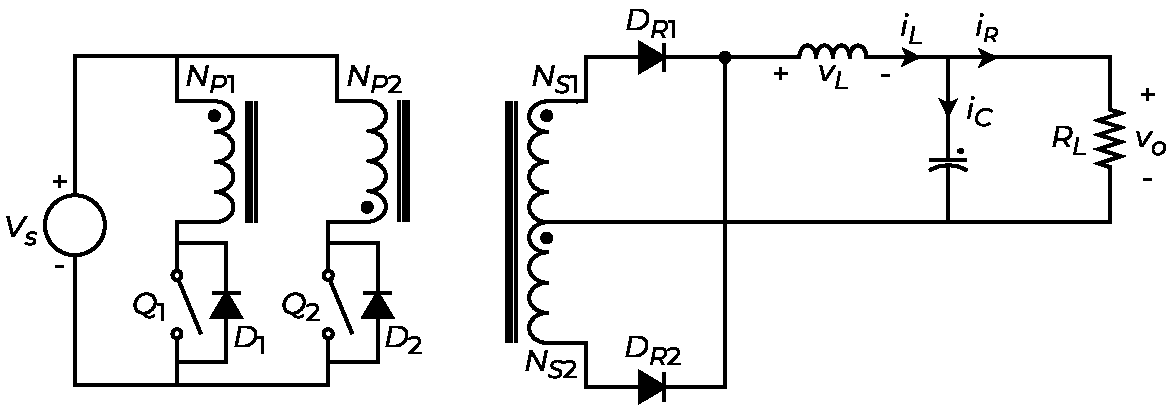
\includegraphics[scale=0.6]{Imagenes/Push-Pull.pdf}
    \caption{Diagrama del convertidor CC-CC de tipo puente completo a utilizar, con todos sus componentes (Placeholder).}
    \label{puente_completo}
\end{figure}

\subsubsection{Especificaciones de Diseño}

La plataforma experimental va a ser utilizada para la evaluación de un módulo de pilas de combustible de \SI[]{300}[]{\watt} de potencia nominal, entregando \SI[]{36}[]{\volt} a \SI[]{8.3}[]{\ampere} de corriente. La tensión de salida varía desde \SI[]{65}[]{\volt} a circuito abierto hasta \SI[]{30}[]{\volt} para la máxima corriente de \SI[]{9.5}[]{\ampere}.\textsuperscript{\cite{HSeriesBrochure}}\\

Esta potencia debe ser transferida por el convertidor hacia la carga variable a la salida, que emula distintas condiciones de carga del bus común de corriente continua de \SI[]{75}[]{\volt} fijos. Dada la potencia de \SI[]{300}[]{\watt}, y si la tensión de salida es la del bus común, entonces el sistema debe soportar una corriente de salida máxima de alrededor de \SI[]{4}[]{\ampere}. Adicionalmente, las llaves del primario van a conmutar a una frecuencia de conmutación de \SI[]{20}[]{\kilo\hertz}, y se debe reducir lo más posible las pérdidas de energía por conmutación, para darle una mayor escalabilidad al diseño.\\

\begin{itemize}
    \item {\SemiBold Potencia nominal \textit{P\textsubscript{N}}:}\quad\SI[]{300}[]{\watt}
    \item {\SemiBold Tensión de salida \textit{v\textsubscript{o}}:}\quad\SI[]{75}[]{\volt}
    \item {\SemiBold Corriente de salida \textit{i\textsubscript{o}}:}\quad\SI[]{4}[]{\ampere}
    \item {\SemiBold Tensión de entrada \textit{v\textsubscript{FC}}:}\quad\SI[]{65}[]{\volt}\textsubscript{máx} , \SI[]{30}[]{\volt}\textsubscript{mín}
    \item {\SemiBold Corriente de entrada \textit{i\textsubscript{FC}}:}\quad\SI[]{9.5}[]{\ampere}
    \item {\SemiBold Frecuencia de conmutación \textit{f\textsubscript{s}}:}\quad\SI[]{20}[]{\kilo\hertz}\\
\end{itemize}

Entonces, con todas estas características quedan definidas las especificaciones necesarias para comenzar la selección y dimensionamiento de componentes del convertidor. Se va a tratar el diseño de cada componente uno por uno, comenzando por los cuatro transistores de potencia que se encargan de la conmutación.\\

\subsubsection{Selección de Llaves}

Las cuatro llaves ideales que conforman el circuito puente del lado primario son implementadas por algún dispositivo electrónico de tres terminales (los dos terminales de potencia, y un tercer terminal de control con el que se comanda la conmutación de la llave). Existen dentro de estas llaves dos categorías distintas: las \textit{llaves semicontroladas}, donde la llave no se puede controlar completamente (por ejemplo se puede comandar el cierre pero no la apertura) y las \textit{llaves completamente controladas} que, como su nombre dice, pueden ser cerradas y abiertas mediante su tercer terminal.\\

En nuestro caso, la topología de puente completo exige la apertura y cierre de las cuatro llaves a la frecuencia de conmutación, por lo que se requieren {\Medium llaves completamente controladas}, dentro de las cuales se pueden elegir una serie de transistores o tiristores.\\

\paragraph{Tecnologías de Transistores}

En nuestro caso, nos vamos a enfocar únicamente en los tres tipos distintos de transistores de potencia, evaluandolos para su uso en la plataforma: el transistor bipolar o BJT (\textit{Bipolar Junction Transistor}), el transistor IGBT (\textit{Insulated-Gate Bipolar Transistor}) y el transistor de efecto de campo o MOSFET (\textit{Metal-Oxide-Semiconductor Field-Effect Transistor}).\\

\subparagraph{Transistor Bipolar}

El transistor bipolar de la figura \ref{bjt} cuenta con su terminal de control, la \textit{base} (B), y sus dos terminales de potencia, el \textit{colector} (C) y \textit{emisor} (E). Este dispositivo se controla mediante la inyección de corriente por la base, por lo que se puede decir que es una llave controlada por corriente.\\

\begin{figure}[h]
    \centering
    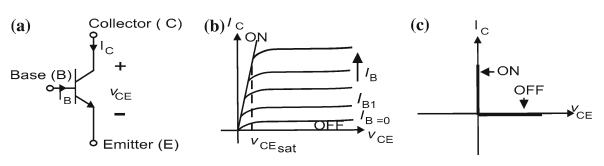
\includegraphics[scale=0.6]{Imagenes/BJT.png}
    \caption{El transistor bipolar (a) su símbolo eléctrico, (b) su curva característica, (c) su curva como llave ideal.}
    \label{bjt}
\end{figure}

Su funcionamiento viene dado por las curvas de corriente de colector $I_C$ contra tensión colector-emisor $V_{CE}$ en el primer cuadrante. El transistor se encuentra en su estado apagado (región de corte) en el área debajo de la curva de corriente de base $I_B$ nula; mientras que se encuentra encendido (región de saturación) en el área donde la tensión $V_{CE}$ es menor a la tensión de saturación ($V_{CE} \leq {V_{CE}}_{sat}$).\\

Hoy en día, los BJT rara vez son utilizados como llaves de potencia, ya que las otras dos tecnologías tienen grandes ventajas frente a este tipo de dispositivo. Primero, al ser un dispositivo controlado por corriente, estos transistores pierden mucha energía de forma disipativa al ser conmutados. Además, al ser un dispositivo de portadores minoritarios, su tiempo de conmutación se ve afectado, cayendo en el orden de los \unit[]{\micro\second}. Sin embargo, como ventaja tienen su baja impedancia de salida, lo que les da una muy baja pérdida de conducción.\textsuperscript{\cite{PotenciaHart}\cite{PowerElecRenewableEnergySystems}}\\

\subparagraph{MOSFET}

El MOSFET de la figura \ref{mosfet} tiene al \textit{gate} (G) como terminal de control, y los terminales de \textit{drain} (D) y \textit{source} (S) como terminales de potencia. Este transistor se controla mediante la variación de la tensión gate-source $V_{GS}$, por lo que, a diferencia del BJT, es un dispositivo controlado por tensión.\\

\begin{figure}[h]
    \centering
    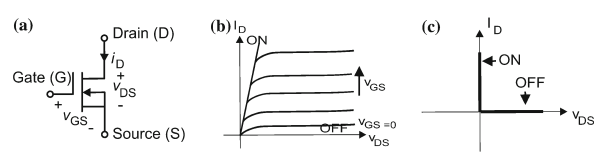
\includegraphics[scale=0.6]{Imagenes/MOSFET.png}
    \caption{El MOSFET (a) su símbolo eléctrico, (b) su curva característica, (c) su curva como llave ideal.}
    \label{mosfet}
\end{figure}

Su funcionamiento es caracterizado por las curvas de corriente de drain $I_D$ versus tensión drain-source $V_{DS}$ en el primer cuadrante. Para encontrarse en estado apagado o región de corte, la tensión de control $V_{GS}$ debe ser menor a una tensión umbral o \textit{threshold} $v_T$ que depende del dispositivo (esto corresponde a la región debajo de la marca OFF en la figura). Cuando la tensión de control supera este umbral, el dispostivo entra en conducción, con una resistencia drain-source ${R_{DS}}_{on}$ baja de orden de \unit[]{\milli\ohm}.\\

Los MOSFET tienen varias características que los hacen deseables como interruptores electrónicos de potencia: al ser controlados por tensión, la pérdida disipativa de potencia para la conmutación es muy baja; como el dispositivo trabaja con portadores mayoritarios, su velocidad de conmutación es muy rápida, con tiempos de conmutación en el orden de los \unit[]{\nano\second}; y tienen una alta impedancia de entrada. Además, por su construcción, tienen un diodo antiparalelo incluido entre D y S, cosa que es deseable para muchas topologías de convertidores.\\

Sin embargo, tienen como desventaja una limitación en tensión y corriente, ya que no soportan corrientes que excedan los \SI[]{200}[]{\ampere} ni tensiones por encima de \SI[]{1}[]{\kilo\volt}; además de tener una elevada impedancia de salida, generando pérdidas de conducción.\textsuperscript{\cite{PotenciaHart}\cite{PowerElecRenewableEnergySystems}}\\

\subparagraph{IGBT}

Los transistores del tipo IGBT podrían ser considerados como un híbrido entre las dos tecnologías anteriores, combinando las ventajas de ambos. Este dispositivo tiene un terminal de control llamado gate (G) al igual que el MOSFET, y dos terminales de potencia, el colector (C) y emisor (E), al igual que el BJT. Se controla mediante la tensión gate-emisor $V_{GE}$, por lo que es controlado por tensión al igual que el MOSFET.\\

\begin{figure}[h]
    \centering
    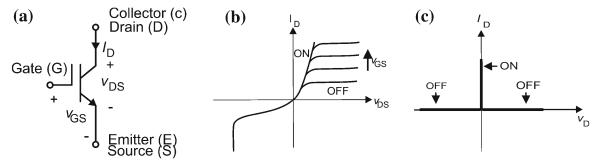
\includegraphics[scale=0.6]{Imagenes/IGBT.png}
    \caption{El IGBT (a) su símbolo eléctrico, (b) su curva característica, (c) su curva como llave ideal.}
    \label{igbt}
\end{figure}

Se caracteriza por la curva de corriente de colector $I_C$ contra tensión gate-emisor $V_{GE}$ de la figura \ref{igbt}, y a diferencia de los anteriores dos transistores, opera en los cuadrantes primero y segundo, es decir que puede bloquear tensión bidireccionalmente y conducir corriente de forma unidireccional.\\

Este transistor combina las ventajas de los BJT y los MOSFET, es decir que tiene una alta impedancia de entrada como el MOSFET, disminuyendo las pérdidas disipativas de la conmutación; una baja impedancia de salida como el BJT, disminuyendo las pérdidas de conducción; y soporta muy altas tensiones, por encima de \SI[]{1}[]{\kilo\volt}, y corrientes mayores a \SI[]{500}[]{\ampere}. Sin embargo, si bien su velocidad de conmutación es superior a la del transistor bipolar, pero no alcanza los cortos tiempos del orden de \unit[]{\nano\second} de los MOSFET, además de ser la tecnología más costosa dentro de las presentadas.\textsuperscript{\cite{PotenciaHart}\cite{PowerElecRenewableEnergySystems}}\\

\paragraph{Selección de MOSFET}

Como las llaves de la plataforma de evaluación nunca excederán los \SI[]{15}[]{\ampere}, y la tensión sobre las llaves no puede superar los \SI[]{70}[]{\volt}, los transistores del tipo MOSFET son la elección más lógica. Sus límites de tensión y corriente están muy por encima de los requierimientos de este diseño, tienen la velocidad de conmutación más rápida y son más económicos que los IGBT. SI bien sus pérdidas de conducción son elevadas, para aplicaciones de relativamente baja potencia como la de este proyecto, se pueden conseguir modelos con muy bajara resistencia de salida ${R_{DS}}_{on}$, mitigando la mayor desventaja de esta tecnología.\\

Entonces, habiendo seleccionado una tecnología de llave, ahora debemos elegir un modelo particular de MOSFET que satisfaga los parámetros necesarios para ser utilizado en el puente de transistores del convertidor. Las características que debe cumplir son:\\

\begin{itemize}
    \item Tensión drain-source $V_{DS} > \SI[]{65}[]{\volt}$, dado que cada transistor debe soportar tensión igual a ${v_{FC}}_{max}$.
    \item Corriente de drain continua $I_D > \SI[]{10}[]{\ampere}$, que es la corriente máxima que es capaz de entregar el modulo de pila de combustible.
    \item Potencia de disipación $P_D > \SI[]{75}[]{\watt}$, ya que la potencia nominal de \SI[]{300}[]{\watt} se distribuye entre las cuatro llaves.
    \item Tiempo de \textit{rise} $t_r$ y \textit{fall} $t_f$ mucho menor al tiempo de un período $T_s = 1/f_s = \SI[]{50}[]{\micro\second}$.
    \item Resistencia de salida ${R_{DS}}_{on}$ lo más baja posible.
    \item Encapsulado \textit{through-hole} capaz de manejar altas disipaciones de potencia.\\
\end{itemize}

Con esto en cuenta, se debe buscar en catálogos y leer especificaciones en hojas de datos para elegir un modelo que cumpla con estas características. Consultando en comerciantes locales y en páginas internacionales como Mouser o DigiKey, se llegó a la familia IRFP de MOSFETs de potencia, con una amplia selección de corrientes y tensiones máximas.\\

Particularmente, se eligió el modelo {\Medium IRFP150N de International Rectifier} (hoy en día parte de Infineon Technologies), cuyas especificaciones se muestran en la siguiente tabla. Estos dispositivos se eligieron por su bajo tiempo de conmutación y resistencia de salida, además fue un factor adicional la disponibilidad de los mismos en el instituto, eliminando la necesidad de comprarlos.\\

\setlength{\tabcolsep}{7pt}
\renewcommand{\arraystretch}{1.5}
\begin{table}[h]
\begin{center}
    \begin{tabular}{lrrrrrrr}
    {\SemiBold Modelo} & $\mathbf{V_{DS}}$ [\unit{\volt}] & $\mathbf{I_D}$ [\unit{\ampere}] & $\mathbf{P_D}$ [\unit{\watt}] & $\mathbf{{R_{DS}}_{on}}$ [\unit{\milli\ohm}] & $\mathbf{t_{on}}$ [\unit{\nano\second}] & $\mathbf{t_{off}}$ [\unit{\nano\second}] & $\mathbf{{V_{GS}}_{th}}$ [\unit{\volt}]\\
    \hline
    IRFP150N & \num{100} & \num{42} & \num{160} & \num{36} & \num{67} & \num{85} & \num{4}
    \end{tabular}
    \caption{Especificaciones del MOSFET de potencia IRFP150N de International Rectifier.\textsuperscript{\cite{DatasheetIRFP150}}}
    \label{tabla:IRFP150}
\end{center}
\end{table}

Donde $V_{DS}$ es la tensión de ruptura drain-source, $I_D$ es la máxima corriente continua de drain, $P_D$ es la máxima disipación de potencia, ${R_{DS}}_{on}$ la resistencia drain-source en estado encendido, $t_{on}$ y $t_{off}$ el tiempo de encendido y apagado, y ${V_{GS}}_{th}$ la tensión umbral para el encendido del transistor.\\

Este transistor es un nMOSFET (canal N) de enriquecimiento de tecnología HEXFET, que tiene incluido en su interior el diodo antiparalelo necesario para la topología de convertidor en uso. Como se puede ver en las especificaciones, cumple con todos nuestros requerimientos: soporta tensiones, corrientes y potencias muy por encima de las requeridas (dando un buen margen de seguridad); una resistencia de conducción muy baja, resultando en pérdidas de menos de \SI[]{0.5}[]{\watt} en cada transistor para \SI[]{10}[]{\ampere} de corriente; y tiempos de encendido y apagado más de cien veces menor al $T_s$ de \SI[]{50}[]{\micro\second}.\\

\begin{figure}[h]
    \centering
    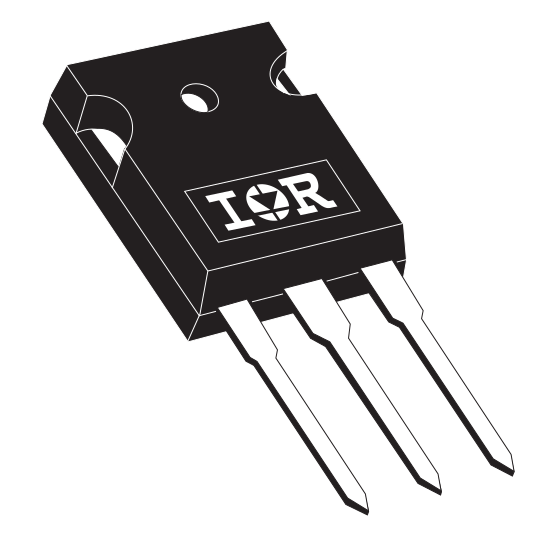
\includegraphics[scale=0.15]{Imagenes/IRFP150-TO247AC.png}
    \caption{MOSFET IRFP150N con su encapsulado THT de potencia tipo TO-247AC.}
    \label{irfp150}
\end{figure}

El encapsulado es del tipo TO-247AC, visible en la figura \ref{irfp150}. Este es un encapsulado through-hole o THT utilizado para dispositivos de alta disipación de potencia, por su tamaño y su superficie metálica que facilita la utilización de un disipador para mantener la temperatura bajo control.\\

\subsubsection{Transformador}

\lipsum[3]\\

\lipsum[4]\\

\subsubsection{Selección de Diodos Rectificadores}

Ahora debemos seleccionar los cuatro diodos que conforman el rectificador de puente completo en el secundario del convertidor. Al igual que los transistores de la sección anterior, estos deben ser diodos de potencia capaces de manejar la potencia de \SI[]{300}[]{\watt} que circulará a través de ellos. Se enumeran a continuación los requerimientos que deben cumplir los diodos seleccionados:\\

\begin{itemize}
    \item Tensión inversa $V_R > \SI[]{150}[]{\volt}$.
    \item Corriente directa $I_F > \SI[]{4.5}[]{\ampere}$.
    \item Tiempo de recuperación de inversa $t_{rr}$ mucho menor al período de conmutación $T_s$ de \SI[]{50}[]{\micro\second}.
    \item Encapsulado THT capaz de manejar altas disipaciones de potencia.\\
\end{itemize}

Con estas especificaciones en cuenta, se eligieron los diodos ultrafast recovery de la serie MUR, particularmente el modelo MUR860 por su corto tiempo de recuperación inversa, baja caída de tensión en conducción y alta tensión inversa máxima. Se detallan sus especificaciones importantes en el siguiente cuadro.\\

\setlength{\tabcolsep}{7pt}
\renewcommand{\arraystretch}{1.5}
\begin{table}[h]
\begin{center}
    \begin{tabular}{llrrrr}
    {\SemiBold Fabricante} & {\SemiBold Modelo} & $\mathbf{V_{RRM}}$ [\unit{\volt}] & $\mathbf{I_{F(AV)}}$ [\unit{\ampere}] & $\mathbf{V_F}$ [\unit{\volt}] & $\mathbf{t_{rr}}$ [\unit{\nano\second}]\\
    \hline
    ON Semiconductor & MUR860 & \num{600} & \num{8} & \num{1.5} & \num{60}\\
    \end{tabular}
    \caption{Especificaciones del diodo rectificador ultrafast recovery MUR860 de ON Semiconductor.\textsuperscript{\cite{MUR860}}}
    \label{tabla:MUR860}
\end{center}
\end{table}

Donde $V_{RRM}$ es la máxima tensión inversa repetitiva, $I_{F(AV)}$ es la máxima corriente rectificada promedio, $V_F$ es la tensión directa instantánea y $t_{rr}$ el máximo tiempo de recuperación inversa.\\

Estos son diodos rectificadores de potencia de la gama ultrafast recovery, pensados para aplicaciones en fuentes de corriente continua conmutadas, como es el caso de este convertidor. Como se ve en el cuadro \ref{tabla:MUR860}, este diodo tiene una tensión inversa máxima muy por encima de los requerimientos, al igual que la máxima corriente directa, que es cerca del doble de lo requerido, dando buenos márgenes de seguridad. Su tiempo de recuperación es similar a los tiempos de conmutación de los transistores IRFP150N de la tabla \ref{tabla:MUR860}, y su caída de tensión en directa de \SI[]{1.5}[]{\volt} es adecuadamente baja.\\

\begin{figure}[h]
    \centering
    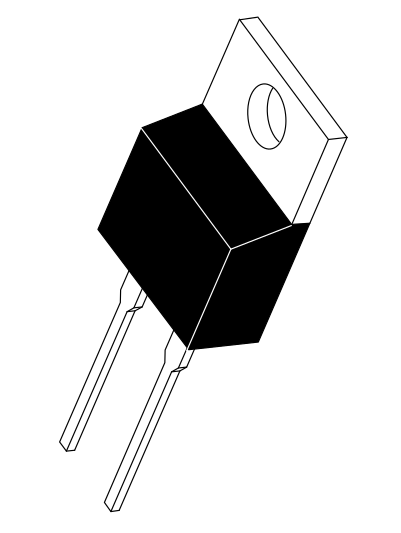
\includegraphics[scale=0.18]{Imagenes/MUR860.png}
    \caption{Diodo rectificador MUR860 con su encapsulado THT de potencia tipo TO-220AC.}
    \label{mur860}
\end{figure}

Se observa este diodo en su encapsulado THT de potencia tipo TO-220AC en la figura \ref{mur860}. Al igual que el encapsulado de los transistores IRFP150N, el TO-220AC posee una superficie metálica en contacto directo con el semiconductor interno que facilita la transferencia de calor hacia un disipador metálico.\\

\subsubsection{Inductor de Salida}

\lipsum[5]\\

\lipsum[6]\\

\subsubsection{Capacitores de Filtro}

\lipsum[7]\\

\lipsum[8]\\

\newpage

\subsection{Circuito Driver}

Como se explicó más arriba, para excitar un transistor MOSFET y encenderlo, es necesario mantener una tensión $V_{GS}$ entre gate y source mayor a una tensión umbral dependiente del modelo. En nuestro caso, esta tensión umbral del IRFP150N es de \SI[]{4}[]{\volt}, como se ve en la tabla \ref{tabla:IRFP150}. Entonces, se debe diseñar algún circuito que sea capaz de proveer estos pulsos de tensión al gate de cada transistor, entregando también la corriente necesaria para cargar y descargar sus capacitancias de gate suficientemente rápido (llamadas corrientes de \textit{source} y \textit{sink}).\\

Este es el llamado {\Medium circuito \textit{driver}} o {\Medium circuito de excitación} y debe existir uno para cada uno de los cuatro transistores del puente. Ahora debemos establecer algunos requerimientos que debe cumplir el circuito:\\

\begin{itemize}
    \item Tensión de operación mayor a \SI[]{100}[]{\volt}, por encima de la máxima tensión de la pila de combustible.
    \item Tiempos de encendido y apagado mucho menores al período $T_s$ de \SI[]{50}[]{\micro\second} de la excitación.
    \item Corrientes de sink y source mayores a \SI[]{2}[]{\ampere} para cargar rápidamente las capacitancias de los transistores, calculado según la nota de aplicación de \cite{SinkSourceCurrent}.
    \item Se busca utilizar una solución integrada, ya que suelen ser más compactas y sencillas.
    \item Es deseable el uso de componentes de montaje superficial o SMD.\\
\end{itemize}

Con estos datos vamos a seleccionar y diseñar un circuito de excitación y explicar brevemente el funcionamiento de todas sus partes.\\

\subsubsection{Selección y Diseño}

Existen diversos tipos de soluciones integradas para circuitos de excitación de transistores MOSFET. Se pueden encontrar circuitos de uno o múltiples canales; existen circuitos que incluyen una aislación entre las entradas y salidas; entre otras funcionalidades. También se consiguen con distintas funciones de seguridad y protección, como el \textit{dead-time}, que permite forzar un tiempo fijo entre la activación de dos transistores de la misma rama, evitando situaciones de cortocircuito; y el \textit{undervoltage lockout} (UVLO), que evita daños por condiciones de baja tensión.\\

Entre todas las opciones, originalmente se había decidido por el modelo UCC21540 de Texas Instruments, un driver de doble canal, con aislación incluida, funcionalidades de dead-time y UVLO, alta capacidad de corriente y un encapsulado SMD de tipo SOIC-16.\\

Sin embargo, este dispositivo no se pudo obtener por falta de disponibilidad, por lo que se tuvo que buscar una alternativa de características similares que esté en disponibilidad. Se terminó decidiendo por el integrado {\Medium 2ED21834-S06J de Infineon Technologies}, cuyas especificaciones básicas se muestran a continuación.\\

\setlength{\tabcolsep}{7pt}
\renewcommand{\arraystretch}{1.5}
\begin{table}[h]
\begin{center}
    \begin{tabular}{llrrrr}
    {\SemiBold Fabricante} & {\SemiBold Modelo} & $\mathbf{V_S}$ [\unit{\volt}] & $\mathbf{I_{OH}/\mathbf{I_{OL}}}$ [\unit{\ampere}] & $\mathbf{t_{on}}/\mathbf{t_{off}}$ [\unit{\nano\second}] & $\mathbf{V_{cc}}$ [\unit{\volt}]\\
    \hline
    \makecell[l]{Infineon \\ Technologies} & 2ED21834-S06J & \num{650} & \num{2.5} & \num{200} & \num{10}-\num{20}
    \end{tabular}
    \caption{Especificaciones del driver modelo 2ED21834-S06J de Infineon Technologies.\textsuperscript{\cite{DatasheetDriver}}}
    \label{tabla:driver}
\end{center}
\end{table}

Donde $V_S$ es la máxima tensión común de operación, $I_{OH}$ e $I_{OL}$ son las corrientes máximas de source y sink, $t_{on}$ y $t_{off}$ son los tiempos de encendido y apagado, y $V_{cc}$ es el rango de tensiones de alimentación.\\ 

El 2ED21834-S06J es un driver de doble canal para medios puentes de transistores de tipo MOSFET e IGBT, con diodo y resistencia de bootstrap incluidos además de funcionalidad de dead-time y UVLO para circuitos del lado bajo y alto, todo contenido en un encapsulado SMD de catorce pines del tipo DSO-14 (figura \ref{encapsulado_driver}). Sus corrientes sink y source de \SI[]{2.5}[]{\ampere} superan la corriente necesaria calculada para los IRFP150N de la tabla \ref{tabla:IRFP150}, su tensión de operación se encuentra cómodamente por encima de la tensión de operación del primario del convertidor, además de tener muy bajos tiempos de conmutación.\\

\begin{figure}[h]
    \centering
    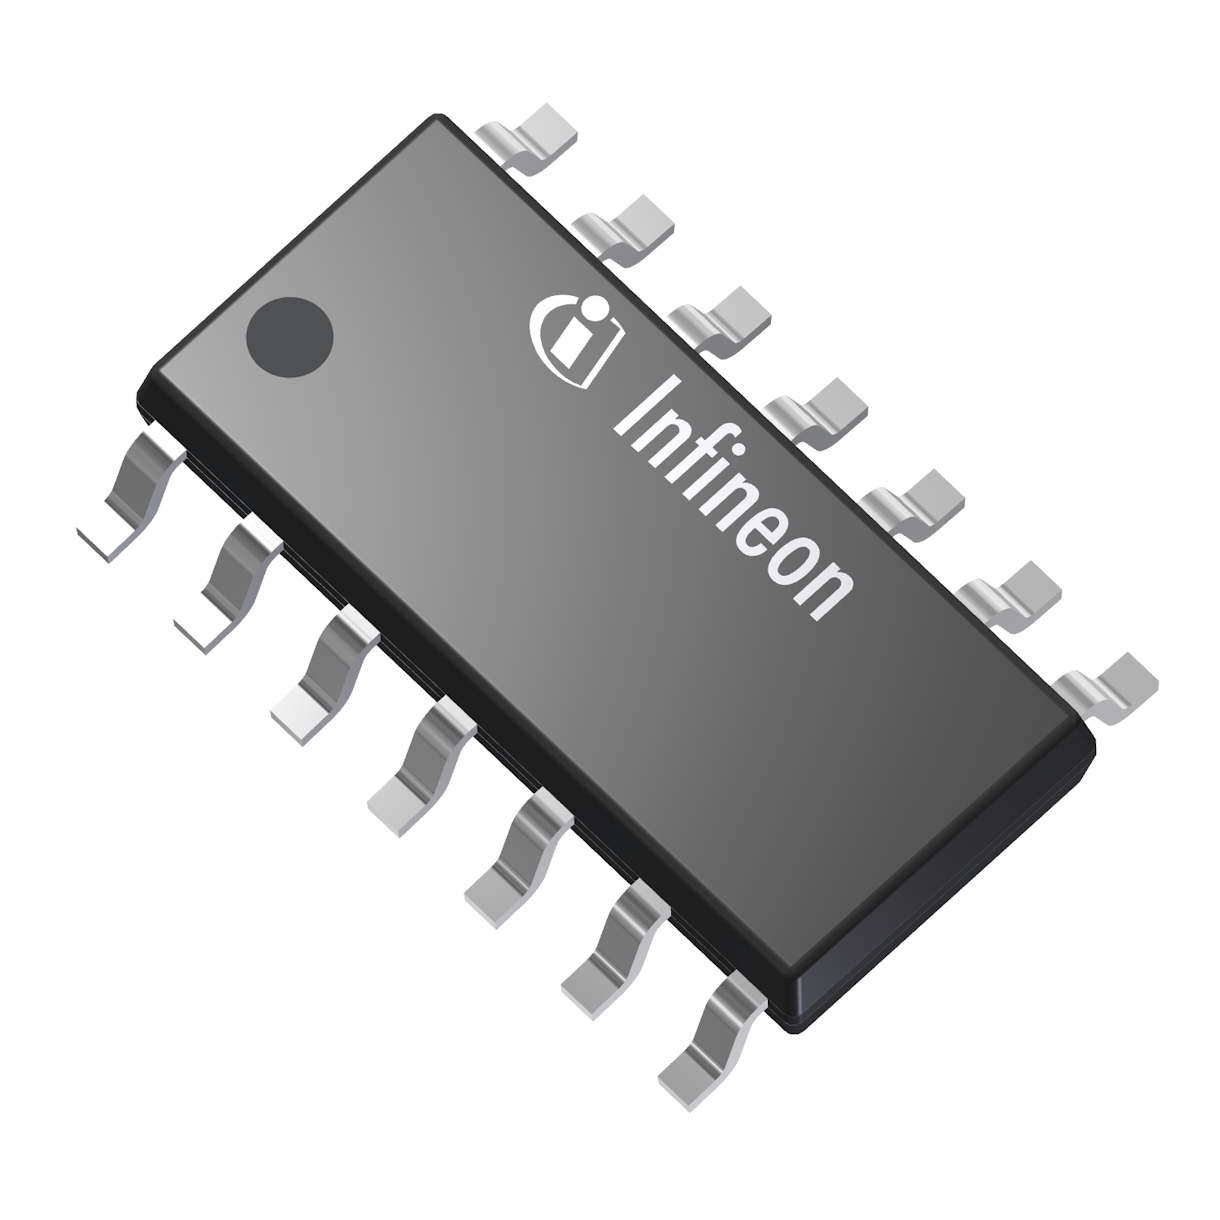
\includegraphics[scale=0.07]{Imagenes/Driver DSO-14.png}
    \caption{Driver 2ED21834-S06J con su encapsulado SMD tipo DSO-14.}
    \label{encapsulado_driver}
\end{figure}

En nuestro caso, se deben utilizar dos de estos dispositivos, uno para cada columna del puente completo. Vamos a utilizar la función de dead-time, configurable mediante una resistencia conectada al pin DT, para proteger contra posibles cortocircuitos causados por la activación errónea de ambos transistores de una columna simultáneamente (\textit{shoot-through}). El resto de la conexión de componentes del driver se realizó de acuerdo a las recomendaciones del fabricante encontradas en la hoja de datos \cite{DatasheetDriver}, que se puede ver en la figura \ref{circuito_driver}.\\

\begin{figure}[h]
    \centering
    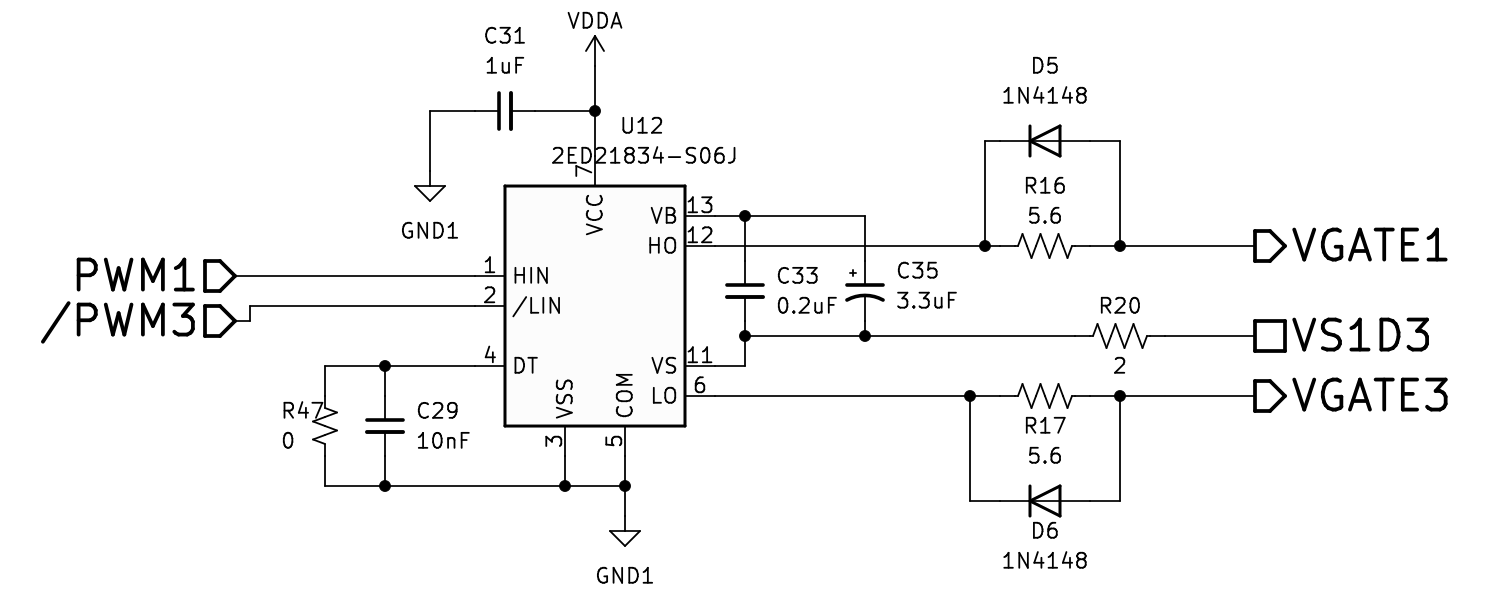
\includegraphics[scale=0.95]{Imagenes/Circuito Driver.png}
    \caption{Circuito de conexión del driver 2ED21834-S06J. El circuito del driver para la otra columna es idéntico.}
    \label{circuito_driver}
\end{figure}

Aquí se puede ver el driver, indicado por la referencia U12, al que le llegan las señales de comando PWM a sus pines HIN y /LIN para el transistor del lado alto y bajo de la columna respectivamente (al estar negada  la entrada para el transistor bajo, la señal que le llega debe estar invertida). Luego, conectado entre el pin DT y tierra se encuentra la resistencia de dead-time, que cuyo valor define el dead-time o tiempo muerto $t_{DT}$. En la salida, se conecta a los pines HO (alto) y LO (bajo) una resistencia limitadora en paralelo con un diodo que permite la descarga de las capacitancias de los transistores, y entre los pines VB y VS se coloca el capacitor que completa el circuito de bootstrap, que se explicará mas adelante. En lo que hace referencia a conexiones a tierra, este circuito, al estar del lado primario del convertidor, se conecta a la referencia $GND_1$. Según la hoja de datos, la tensión de alimentación debe ser de entre \SI[]{10}[]{\volt} y \SI[]{20}[]{\volt}, por lo que se alimenta con una tensión no regulada de \num{12}-\SI[]{18}[]{\volt}.\\

El dimensionamiento de todos estos componentes se va a tratar a continuación siguiendo las recomendaciones del fabricante disponibles en hojas de datos y notas.

\subsubsection{Dimensionamiento de Componentes}

\lipsum[1]\\

\lipsum[2]\\

\subsubsection{Esquema Interno del Dispositivo}

{\Bold\scshape Falta completar esta sección.}\\

\lipsum[1]\\

\begin{figure}[h]
    \centering
    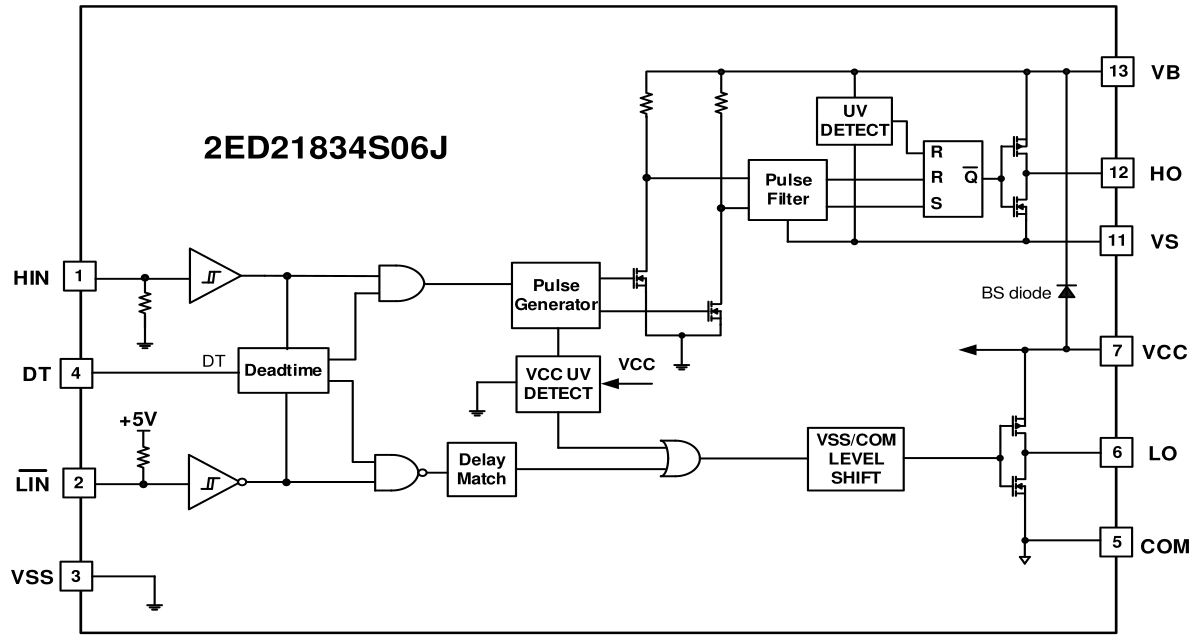
\includegraphics[scale=0.25]{Imagenes/Esquema Interno Driver.png}
    \caption{Diagrama de bloques interno del driver 2ED21834-S06J de Infineon Technologies.}
    \label{interno_driver}
\end{figure}

\lipsum[2]\\

\lipsum[3]\\

\lipsum[4]\\

\newpage

\subsection{Sistema de Medición}

Con lo tratado en la sección del sistema de control del capítulo \ref{analisis}, se estableció que para realizar un adecuado control de la plataforma, se debe tomar información de cuatro variables de estado del sistema: la tensión y corriente de la pila de combustible ($v_{FC}$ e $i_{FC}$) y la tensión y corriente de salida ($v_o$ e $i_o$). En esta sección se va a tratar el diseño del sistema de medición de datos de la figura \ref{diag_medicion}, que incluye el sensado de los parámetros del convertidor, el acondicionamiento de las señales, y la transmisión de las mismas al sistema de control.\\

\begin{figure}[h]
    \centering
    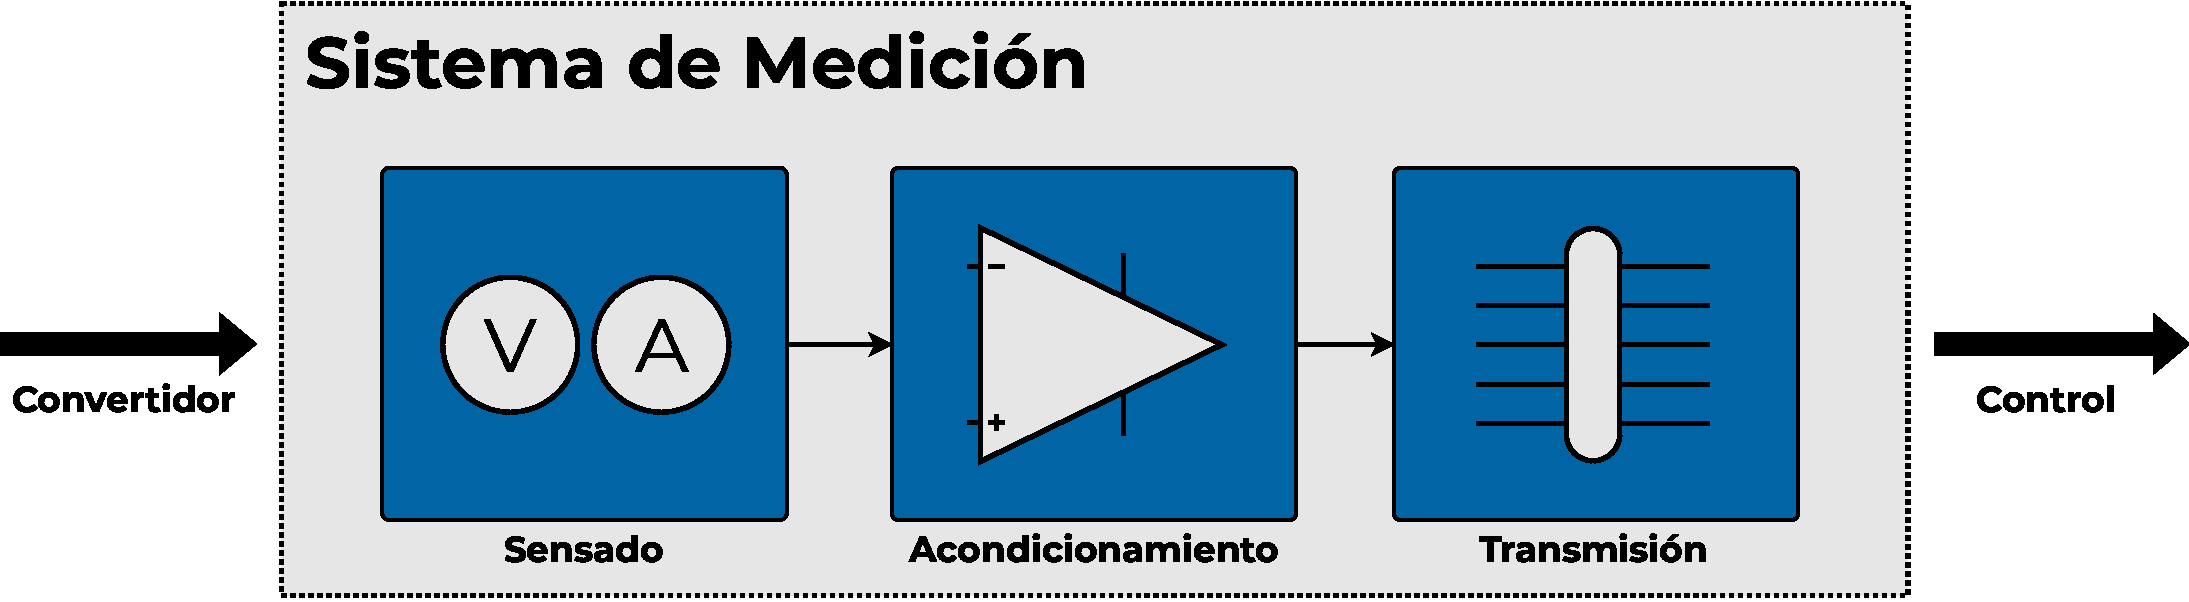
\includegraphics[scale=0.4]{Imagenes/Sistema Medicion.pdf}
    \caption{Sistema de medición de la plataforma, con las tres etapas que lo conforman.}
    \label{diag_medicion}
\end{figure}

Este sistema comienza con la adquisición de los parámetros de interés provenientes del convertidor, tarea llevada a cabo por los sensores de tensión y corriente que conforman la {\Medium etapa de sensado}. Sin embargo, estos datos obtenidos no se presentan en una forma que nuestro sistema de control sea capaz de procesar, por lo que se necesita la siguiente etapa del sistema, la {\Medium etapa de acondicionamiento}, que se encarga de adecuar los datos obtenidos por los sensores para que puedan ser utilizados por el controlador. Finalmente, necesitamos una forma de llevar estos datos desde el sistema de medición hasta el controlador, función que es llevada a cabo por el último bloque de la figura, la {\Medium etapa de transmisión}.\\

Vamos a tratar el diseño de este sistema en el orden que se observa en la figura, por lo que se comenzará por la etapa de sensado o adquisición de datos.\\

\subsubsection{Etapa de Sensado}

En este sistema, los únicos parámetros a medir son tensiones y corrientes, tanto de la pila de combustible a la entrada como de la carga variable a la salida. Previamente a la seleccion de los sensores a utilizar, vamos a realizar una breve categorización y explicación de los métodos de sensado disponibles para ambos parámetros, comenzando por las tensiones.\\

\paragraph{Tecnologías de Sensado de Tensión}

Este es el más simple de los dos casos, ya que los sistemas de control ya trabajan con señales expresadas en tensiones, por lo que no es requerido ningún tipo de transductor, únicamente una adaptación de niveles que es llevada a cabo por la etapa de acondicionamiento. Por esta razón, lo único necesario en este caso es la obtención directa de la tensión buscada, siempre minimizando la perturbación que esta medición introduce al sistema.\\

\paragraph{Tecnologías de Sensado de Corriente}

A diferencia del caso de las tensiones, para poder obtener una medición de corriente se debe realizar algún tipo de transducción que transforme la información de corriente en valores de tensión que puedan ser utilizados por el sistema de control. Existen múltiples tecnologías de sensado y transucción de corriente fundamentalmente distintas, cada una con sus propias características, ventajas y desventajas. Vamos a dedicar algunos párrafos a su clasificación y descripción.\\

\subparagraph{Resistencia Shunt}

Es el método conceptualmente más sencillo de todos, y consiste en interponer al camino de la corriente un resistor \textit{shunt} $R_S$, es decir una resistencia de muy bajo valor (generalmente en las decenas y unidades de \unit{\milli\ohm}), y luego medir la caída de tensión en el mismo. Esta corriente se encuentra directamente relacionada con la tensión mediante la Ley de Ohm, que luego de reordenar resulta:

\begin{equation}\label{ec_shunt}
    I=\frac{1}{R_S}V_S
\end{equation}

Entonces, con este método se obtiene una relación {\Medium perfectamente lineal} entre entre la tensión medida directamente y la corriente que se quiere obtener, siendo el inverso del valor del resistor (o su conductancia) la constante de proporcionalidad. Al tener la Ley de Ohm como su principio de funcionamiento, este método es capaz de medir todo tipo de corrientes, tanto continua (CC) como alterna (CA). Además, al necesitar únicamente una resistor, es {\Medium sumamente sencillo} de implementar.\\

Sin embargo, al estar circulando toda la corriente a través del resistor, se genera una {\Medium pérdida de energía significativa}, ya que la potencia disipada depende del cuadrado de la corriente. Si tomamos la plataforma como ejemplo, donde la corriente de pila $i_{FC}$ en el primario puede llegar a un máximo de \SI[]{10}[]{\ampere}, una resistencia shunt de \SI[]{50}[]{\milli\ohm} puede llegar a disipar una potencia de \SI[]{5}[]{\watt}. Por esta razón, este método no es factible para mediciones de grandes corrientes.\\

La precisión de este método también se {\Medium deteriora con la frecuencia}, ya que para frecuencias suficientemente altas, los efectos de la inductancia parásita $L_S$ y el efecto skin generan un aumento de la impedancia que afecta a la medición.\\

Dadas las altas potencias que puede llegar a disipar un resistor shunt, la temperatura puede presentar un problema si su coeficiente de temperatura no es adecuado. Los fabricantes de estas resistencias tienen esto en cuenta y fabrican los componentes con materiales de bajo coeficiente de temperatura.\\

\begin{figure}[h]
    \centering
    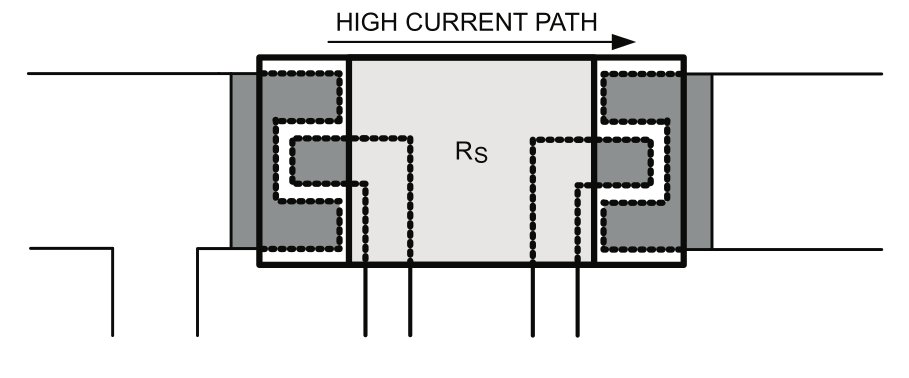
\includegraphics[scale=1.1]{Imagenes/Conexion Kelvin.png}
    \caption{Conexión Kelvin de cuatro cables para el sensado de corriente con un resistor shunt de montaje superficial.}
    \label{conexion_kelvin}
\end{figure}

Sin embargo, esto no puede solucionar el error introducido por el coeficiente de temperatura de las soldaduras, que se exacerban particularmente para valores bajos de resistencia. Para solventarlo, se debe utilizar la conexión de cuatro cables o Kelvin, que separa el camino de alta corriente de las conexiones de sensado, como se ve en la figura \ref{conexion_kelvin}.\textsuperscript{\cite{CurrentSensing}}\\

\subparagraph{Bobina de Rogowski}

Este es un método de medición de corriente basado en la Ley de Inducción de Faraday, y por lo tanto, {\Medium provee aislamiento eléctrico} por su propio principio funcionamiento, a diferencia del método anterior. Este dispositivo consiste, fundamentalmente, en una bobina de forma toroidal y núcleo no ferromagnético a través de la cual se hace pasar el conductor del que se quiere medir la corriente.\\

\begin{figure}[h]
    \centering
    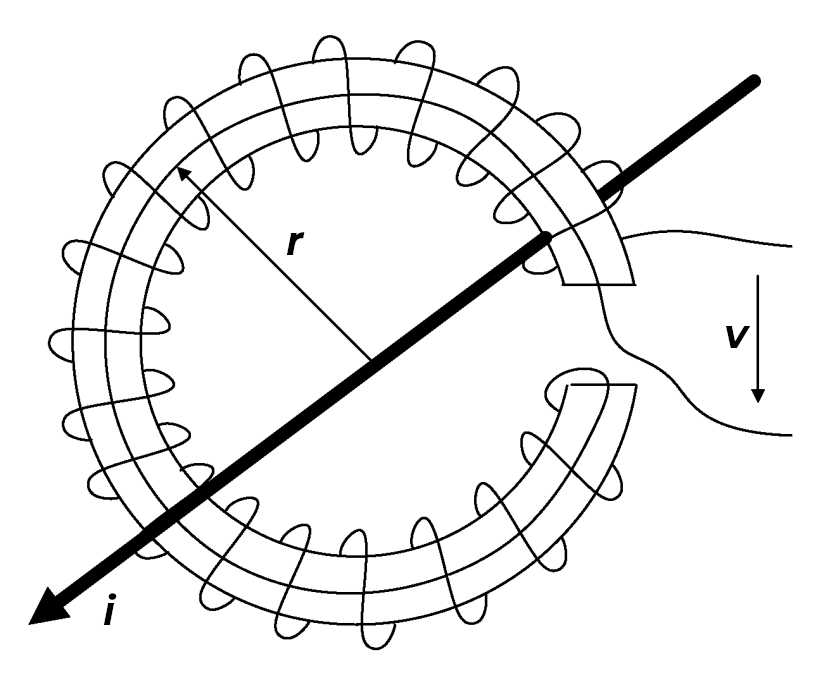
\includegraphics[scale=0.2]{Imagenes/Bobina Rogowski.png}
    \caption{Esquema de una bobina de Rogowski utilizada para medir la corriente $i$ que circula por el conductor.}
    \label{bobina_rogowski}
\end{figure}

Utilizando las leyes de Ampere (que relaciona la integral de un campo magnético en un camino cerrado con la corriente que este encierra) y Faraday (que relaciona la velocidad de cambio de un flujo magnético con la tensión o fuerza electromotriz) se puede obtener una expresión para la tensión medida en bornes de la bobina en función de la corriente de interés. Siguiendo el desarrollo de \cite{CurrentSensing}, se obtiene la siguiente expresión para la tensión de salida.

\begin{equation*}
    v = -\frac{NA\mu_0}{2\pi r}\cdot \frac{di}{dt}
\end{equation*}

Donde $N$ es la cantidad de vueltas de la bobina, $A$ es el área de un corte de la bobina, y $r$ es el radio de la bobina. Sin embargo, en esta ecuación la tensión de salida depende de la velocidad de cambio de la corriente que nos interesa. Entonces, se debe agregar un integrador de constante de integración $k$ a la salida de la bobina, para obtener la tensión $v_o$ dependiente de la corriente que nos interesa.

\begin{equation}\label{ec_rogowski}
    v_o = -k\cdot\frac{NA\mu_0}{2\pi r}\cdot i + v_o(0)
\end{equation}

Una gran ventaja de esta tecnología, es que al no utilizar un núcleo ferromagnético, tiene un rango de medición {\Medium altamente lineal}, comparable con el de una medición por shunt. Además de esto, al no tener que conectar nada al circuito en estudio, prácticamente {\Medium no introduce perturbaciones}, existiendo únicamente pequeños efectos causados por la inductancia de la bobina.\\

Comparado con el resistor shunt, este método presenta muy {\Medium bajas pérdidas} energéticas, al no tener circulación de altas corrientes. Por esta razón, este método es capaz de medir muy {\Medium grandes corrientes}, del orden de los \unit{\mega\ampere}, presentando una clara ventaja respecto al shunt.\\

Sin embargo, al estar su funcionamiento basado en la detección de un cambio de flujo magnético, este sensor es {\Medium incapaz de detectar corrientes continuas}, y tiene dificultades con la detección de componentes de baja frecuencia (es común la utilización de estas bobinas en conjunto con otros sensores capaces de detectar continua).\\

Otra desventaja que dificulta su implementación para nuestra aplicación, es que estas bobinas {\Medium ocupan un gran espacio} y no resulta sencillo integrarlas de forma compacta en una placa de circuito impreso. Además, por esto y por la necesidad de implementar un integrador, su costo es considerable frente al shunt.\\

\subparagraph{Transformador de Corriente}

Al igual que la bobina de Rogowski, este método se aprovecha de los principios establecidos por la ley de inducción de Faraday, por lo que también tiene {\Medium aislación intrínseca}. Su construcción es similar a las bobinas, con una vuelta de bobinado en el primario y una gran cantidad de vueltas en el secundario, pero a diferencia de estas, tiene un núcleo de material ferromagnético. Luego, conectada al secundario se encuentra una resistencia de sensado $R_S$ por la que circula la corriente de secundario $i_s$, generando una caída de tensión $v_s$. Se mide esta tensión, al igual que en el caso del shunt, y se obtiene la corriente del primario en función de esta.

\begin{equation*}
    i = Ni_s + \frac{N}{L_m}\int_t v_s\cdot dt
\end{equation*}

Donde $N$ es la cantidad de vueltas del transformador y $L_m$ es la inductancia magnetizante del transformador. Si reemplazamos la corriente del secundario $i_s$ por la expresión del shunt de la ecuación \ref{ec_shunt}, obtenemos la expresión de la corriente en función de la tensión medida.

\begin{equation}\label{ec_trafocorriente}
    i = N\frac{v_s}{R_S} + \frac{N}{L_m}\int_t v_s\cdot dt
\end{equation}

El término integral de esta ecuación indica que este método es {\Medium incapaz de medir corrientes continuas}: si la corriente $i$ del primario contiene componentes de CC, la corriente magnetizante aumenta hasta que todo el componente de corriente circula únicamente por la inductancia magnetizante $L_m$.\\

Como las vueltas $N$ del secundario pueden ser muy elevadas, se puede obtener una corriente de secundario muy baja, y en consecuencia unas {\Medium bajas pérdidas de energía}. Además, si el término integrador es pequeño (que es el caso para altas frecuencias), las corrientes de primario y secundario son prácticamente proporcionales, resultando en un sensor con {\Medium buena linealidad}.\\

\begin{figure}[h]
    \centering
    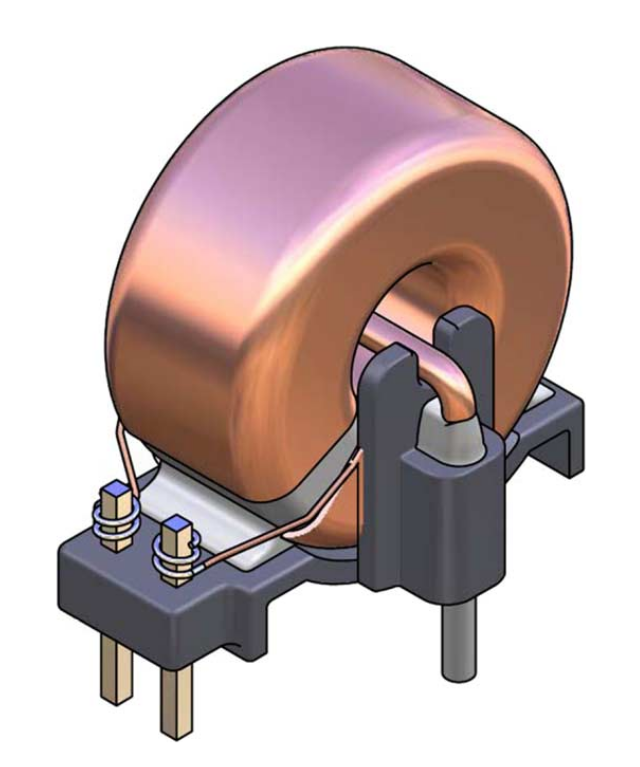
\includegraphics[scale=0.2]{Imagenes/Trafo Corriente.png}
    \caption{Transformador de corriente con una vuelta de primario y múltiples vueltas de secundario.}
    \label{trafo_corriente}
\end{figure}

La inductancia $L_m$ introduce errores de medición, ya que la corriente que circula por ella no circula por la resistencia de sensado, y por lo tanto esto disminuye la caída de tensión $v_s$. Este es un fenómeno conocido como \textit{droop}, y se exacerba particularmente para pulsos de corriente de tiempos largos de encendido en el primario (esto es de interés para nuestra aplicación, dados los pulsos generados por la conmutación de las llaves).\\

Además, como se ve en la figura \ref{trafo_corriente}, su integración en una plaqueta puede ser problemático por su {\Medium gran tamaño}. Sin embargo, hoy en día son muy populares en aplicaciones de convertidores, dado su {\Medium bajo costo} y su salida que suele ser directamente compatible con conversores analógico-digitales.\\

\subparagraph{Efecto Hall}

Finalmente, una tecnología que se utiliza mucho hoy en día son los sensores por efecto Hall, del tipo de medición de campo magnético, basados en el efecto homónimo descubierto por Edwin Hall en 1879. Este efecto consiste en una fina placa metálica sobre la que circula una corriente $I$, atravesada perpendicularmente por un campo magnético $B$, genera una diferencia de potencial $v$ perpendicular a ambos.

\begin{figure}[h]
    \centering
    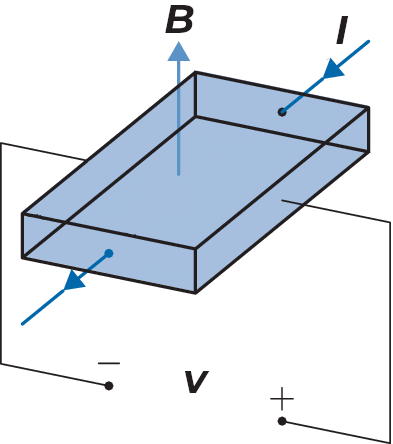
\includegraphics[scale=0.35]{Imagenes/Efecto Hall.png}
    \caption{Diagrama que muestra el principio de funcionamiento de un sensor de corriente por efecto Hall.}
    \label{efecto_hall}
\end{figure}

Entonces, generando un campo magnético que atraviese una placa por la que circula la corriente de interés $i$, se puede medir la tensión que cae en ellas y obtener por medio de esta el valor de la corriente según la ecuación de Hall.

\begin{equation}
    I = v\cdot\frac{nqd}{B}
\end{equation}

Dónde $q$ es la carga de los portadores, $n$ la densidad de portadores y $d$ el grosor de la placa. Como $n$ y $q$ son parámetros que dependen exclusivamente del material utilizado, se suelen consolidar en un parámetro llamado coeficiente de Hall $R_H$, que se define como la inversa del producto de $n$ y $q$. Entonces, la ecuación del sensor resulta:

\begin{equation}\label{ec_hall}
    I = v\cdot\frac{d}{R_HB}
\end{equation}

Como se puede ver por la ecuación, este método posee una {\Medium buena linealidad}, y además, como la corriente circula por un simple conductor, la perturbación introducida es mínima y tiene {\Medium bajas pérdidas de potencia}.\\

Al igual que los métodos de bobina de Rogowski y transformador de corriente, este método, por su principio de funcionamiento, ya {\Medium incluye aislación galvánica}. Pero, a diferencia de los otros métodos magnéticos e inductivos, los sensores de efecto Hall son perfectamente {\Medium capaces de realizar mediciones de corriente continua}.\\

En tanto a sus problemas, los materiales utilizados para las placas metálicas de los sensores suelen tener {\Medium elevadas constantes de temperatura}, por lo que pueden resultar muy susceptibles a cambios de temperatura por sobrecalentamiento. También, para un campo magnético nulo existe una tensión de salida de \textit{offset} no nula, por lo que se requiere electrónica adicional para compensar por este error.\\

Sin embargo, hoy en día existen soluciones integradas en pequeños empaquetados de montaje superficial como los SOIC o SOP, que incluyen un sensor de efecto hall con toda la electrónica asociada necesaria para compensar la tensión de offset y las variaciones por temperatura. Estas son soluciones compactas y de alta precisión, a pesar de su precio mayor comparado con otros métodos.\\\pagebreak

\subparagraph{Resumen}

A modo de resumen de todo lo explicado, se presenta la tabla \ref{tabla:resumen_sensores} que contiene las principales características de interés de las tecnologías de medición de corriente explicadas.\\

\setlength{\tabcolsep}{6pt}
\renewcommand{\arraystretch}{1.5}
\begin{table}[h]
\begin{center}
    \begin{tabular}{l|lllll}
         & {\SemiBold Ancho de Banda} & {\SemiBold Precisión} & \makecell[l]{{\SemiBold Medición} \\ {\SemiBold de CC}} & {\SemiBold Aislación} & {\SemiBold Pérdidas}\\
        \hline
        Shunt & \unit{\kilo\hertz}-\unit{\mega\hertz} & \num{0,1}\% - \num{2}\% & Sí & No & \unit{\milli\watt}-\unit{\watt}\\
        \makecell[l]{Bobina de \\ Rogowski} & \unit{\kilo\hertz}-\unit{\mega\hertz} & \num{0,1}\% - \num{1}\% & No & Sí & \unit{\milli\watt}\\
        Transformador & \unit{\kilo\hertz}-\unit{\mega\hertz} & \num{0,1}\% - \num{1}\% & No & Sí & \unit{\milli\watt}\\
        Efecto Hall & \unit{\kilo\hertz} & \num{0.5}\% - \num{5}\% & Sí & Sí & \unit{\milli\watt}
    \end{tabular}
    \caption{Resumen de las características principales de cada tecnología de sensado de corriente.\textsuperscript{\cite{CurrentSensing}}}
    \label{tabla:resumen_sensores}
\end{center}
\end{table}

Con la información de los distintos tipos de sensores de corriente que se explicaron, se deben seleccionar los modelos de los sensores de la tecnología adecuada para la medición de las variables, buscando en catálogos de sensores.\\

\paragraph{Sensor de Corriente $\mathbf{i_o}$}

La corriente de salida $i_o$ es la variable a medir más importante, ya que es la que directamente controla la potencia de salida que se entrega al bus de continua del sistema híbrido. Por esta razón, debe cumplir algunos requerimientos que se enumeran a continuación.\\

\begin{itemize}
    \item Capacidad de corriente mayor a \SI[]{4.5}[]{\ampere}.
    \item Tensión de operación mayor a \SI[]{100}[]{\volt}.
    \item Precisión de medición debajo del $\pm$1\%.
    \item Ancho de banda $BW$ por encima de \SI[]{40}[]{\kilo\hertz}, el doble de la frecuencia de conmutación.
    \item Capacidad de medir componentes de CC.
    \item Es deseable que el sensor esté galvánicamente aislado del circuito del convertidor.\\
\end{itemize}

La necesidad de medir componentes de corriente continua elimina automáticamente la posibilidad de usar una bobina de Rogowski o un transformador de corriente. Por lo tanto, nos quedan como opciones únicamente la resistencia shunt y el sensor de efecto Hall, que dado que ambos son capaces de precisiones debajo del \num{1}\% y anchos de banda de \unit{\kilo\hertz}, se decide utilizar un {\Medium sensor de efecto Hall}, por la presencia de aislación galvánica.\\

Entonces, buscando sensores de corriente de efecto Hall en catálogos online, se llegó al modelo {\Medium TMCS1100A4} de Texas Instruments, un sensor Hall de medición bidireccional (corrientes positivas y negativas) de alta precisión y aislamiento básico, todo en un encapsulado de montaje superficial de ocho pines tipo SOIC-8. Según la hoja de datos del fabricante, este dispostivo esta pensado para ser utilizado en la medición de corrientes de inversores y puentes completos. Sus especificaciones se presentan en la tabla \ref{tabla:sensor_hall}.\\

\setlength{\tabcolsep}{6pt}
\renewcommand{\arraystretch}{1.5}
\begin{table}[H]
\begin{center}
    \begin{tabular}{llrrrrr}
    {\SemiBold Fabricante} & {\SemiBold Modelo} & $\mathbf{I_{in}}$ [\unit{\ampere}] & $\mathbf{V_{in}}$ [\unit{\volt}] & $\mathbf{BW}$ [\unit{\kilo\hertz}] & $\mathbf{e_i}$ & {\SemiBold Sens.} [\unit{\milli\volt\per\ampere}]\\
    \hline
    \makecell[l]{Texas \\ Instruments} & TMCS1100A4 & \num{12} & \num{600} &  \num{80} & $\pm$\num{0.9}\% & \num{400}
    \end{tabular}
    \caption{Especificaciones del sensor de corriente por efecto Hall, modelo TMCS1100A4 de Texas Instruments.\textsuperscript{\cite{TMCS1100}}}
    \label{tabla:sensor_hall}
\end{center}
\end{table}

Dónde $I_{in}$ es la máxima corriente unidireccional medible, $V_{in}$ es la máxima tensión de operación en la entrada, $BW$ es el ancho de banda de la medición, y $e_i$ es la precisión o error relativo de la medición.\\ 

La variante A4 tiene una sensibilidad de \SI[]{400}[]{\milli\volt\per\ampere}, poniendo la tensión de salida en el rango de \num{0} a \SI[]{1.8}[]{\volt} para una corriente de salida $i_o$ máxima de \SI[]{4.5}[]{\ampere}. Además, si tomamos el error relativo máximo de $\pm$\num{0.9}\%, se obtiene que la precisión absoluta es de $\pm$\SI[]{40}[]{\milli\ampere}, más que suficiente para ser aplicado en la plataforma.\\

\begin{figure}[h]
    \centering
    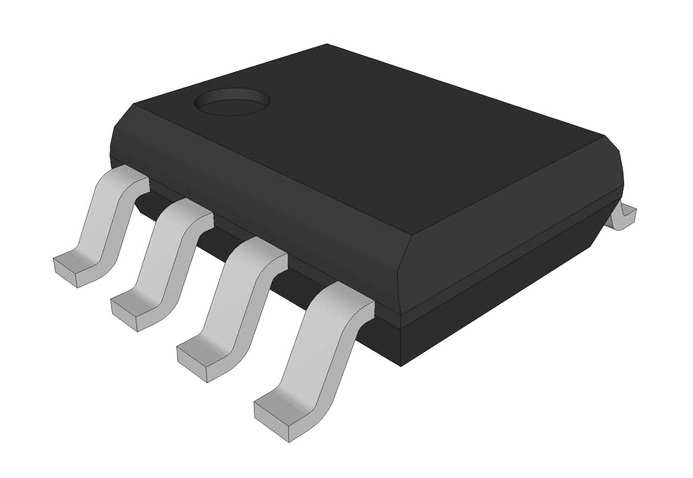
\includegraphics[scale=0.8]{Imagenes/SOIC8.jpg}
    \caption{Sensor de corriente por efecto Hall, modelo TMCS1100A4 de Texas Instruments, en su encapsulado tipo SOIC-8.}
    \label{encapsulado_hall}
\end{figure}

El sensor tiene cuatro pines para el sensado de corriente, dos llamados IN+ y dos llamados IN-. Como se trata de medición de corriente, se debe conectar el sensor en serie al camino de corriente, con la corriente entrando por los pines IN+ y saliendo por los pines IN-.\\

Luego, el pin de tensión de referencia VREF se conecta a masa, que de esta manera configura el sensor para utilizar un rango de medición unidireccional (configurando la tensión de salida nula para corriente nula)\textsuperscript{\cite{TMCS1100}}, ya que en nuestro caso la corriente solo puede circular hacia la carga.\\

\begin{figure}[h]
    \centering
    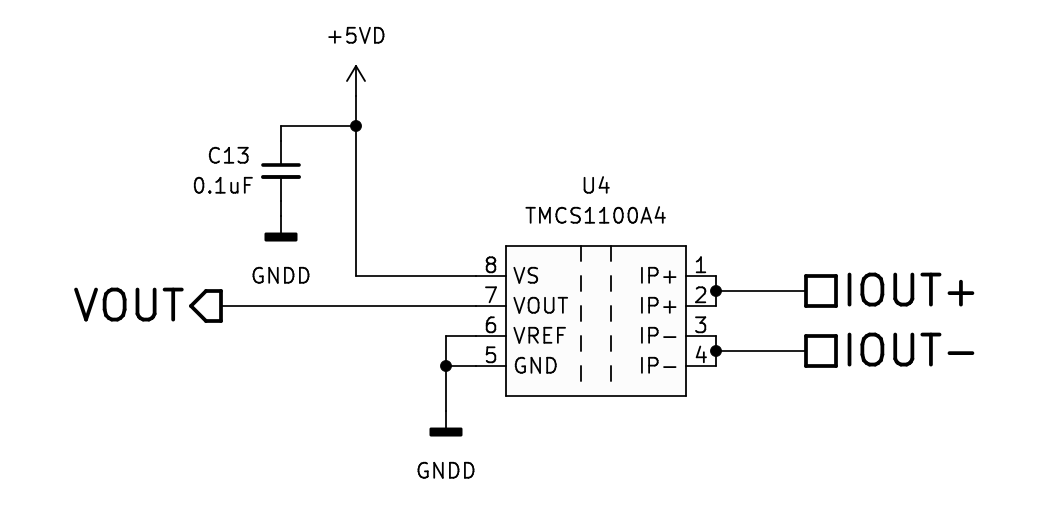
\includegraphics[scale=1]{Imagenes/Conexion TMCS1100.png}
    \caption{Conexión del sensor TMCS1100A4, según recomendaciones del fabricante.}
    \label{conexion_TMCS1100}
\end{figure}

Todas las conexiones a tierra del sensor se realizan en la tierra de señal o digital $GND_D$, ya que se encuentran todas del segundo lado del dispositivo, aislados del circuito de potencia del convertidor. El pin VS se conecta a la alimentación digital del sistema requiriendo una tensión de \SI[]{5}[]{\volt} positivos, con un capacitor de filtro conectado en derivación según recomendación del fabricante.\\

El pin de salida VOUT, como se verá mas adelante, se debe conectar primero a un circuito que acondicione la señal que el sensor arroja, para luego poder ser conectado a la entrada del conversor analógico-digital (ADC) del controlador que convertirá los datos analógicos de corriente en datos digitales que pueda procesar.\\

\paragraph{Sensor de $\mathbf{v_{FC}}$, $\mathbf{i_{FC}}$ y $\mathbf{v_o}$}

Por una cuestión de simplicidad, se eligió buscar una única solución integrada que sea capaz de medir múltiples variables, en nuestro caso una corriente y dos tensiones. Dado que las variables restantes son de menor importancia, limitar el requerimiento de ancho de banda respecto a la corriente de salida. A continuación se detallan algunos requerimientos.\\

\begin{itemize}
    \item Capacidad de medición de corriente por arriba de \SI[]{11}[]{\ampere}.
    \item Capacidad de medición de tensión por arriba de \SI[]{75}[]{\volt}.
    \item Precisión mejor o igual al $\pm$\num{2}\%.
    \item Capacidad de medir componentes de CC.
    \item Ancho de banda $BW$ lo más alto posible.
    \item Es deseable que el sensor esté galvánicamente aislado del circuito del convertidor.\\
\end{itemize}

Buscando en catálogos online de distintos fabricantes se encontró el {\Medium circuito integrado LM5056A} de Texas Instruments, descrito por el fabricante como un \quotes{Dispositivo de Administración de Potencia de Sistemas de Alta Tensión}.\\

Consiste en un sensor de corriente de tipo shunt, junto con un sensor de tensión a la entrada del shunt y una medición de tensión secundaria, con la capacidad adicional de calcular la potencia en base a las mediciones.  Al usar medición de tipo shunt, tiene la capacidad de medir componentes de CC, pero no posee aislación galvánica. Se detallan algunas especificaciones a continuación.\\

\setlength{\tabcolsep}{6pt}
\renewcommand{\arraystretch}{1.5}
\begin{table}[H]
\begin{center}
    \begin{tabular}{llrrrrr}
    {\SemiBold Fabricante} & {\SemiBold Modelo} & $\mathbf{V_{in/out}}$ [\unit{\volt}] & $\mathbf{f_m}$ [\unit{\kilo\hertz}] & $\mathbf{I_{in(FSR)}}$ [\unit{\milli\volt}] & $\mathbf{e_{i}}$ & $\mathbf{e_v}$\\
    \hline
    \makecell[l]{Texas \\ Instruments} & LM5056A & \num{100} & \num{1} &  \num{27}/\num{54.4} & $\pm$\num{1.25}\% & $\pm$\num{1}\%
    \end{tabular}
    \caption{Especificaciones del sensor combinado de tensión, corriente y potencia por shunt, modelo LM5056A de Texas Instruments.\textsuperscript{\cite{LM5056A}}}
    \label{tabla:LM5056A}
\end{center}
\end{table}

Donde $V_{in/out}$ es la máxima tensión de entrada y salida medible, $f_m$ es la frecuencia de muestreo del sensor, $I_{in(FSR)}$ es la tensión de fondo de escala de medición de corriente, $e_i$ es la precisión de la medida de corriente, y $e_v$ es la precisión de la medida de tensión.\\

Los parámetros analógicos de tensión y corriente medidos por el LM5056A son muestreados y convertidos a información digital mediante un conversor analógico-digital interno de \num{12} bits de resolución, (es decir $2^{12} = 4096$ niveles distintos) con frecuencia de muestreo $f_m$ de \SI[]{1}[]{\kilo\hertz} como muestra la tabla. Una vez convertidos, se pueden transmitir mediante la interfaz de bus I\textsuperscript{2}C que provee el integrado, con pines SDAO para salida de datos, SDAI para entrada de datos y SCL para entrada de reloj. Esta interfaz se explica más adelante en la sección 3.4.3, sobre la etapa de transmisión.\\

Este dispositivo viene en un empaquetado de montaje superficial del tipo HTSSOP-28 de veintiocho pines (figura \ref{encapsulado_LM5056}), que también incluye un contacto plano en la parte inferior, de conexión opcional para la disipación de calor.\\

\begin{figure}[h]
    \centering
    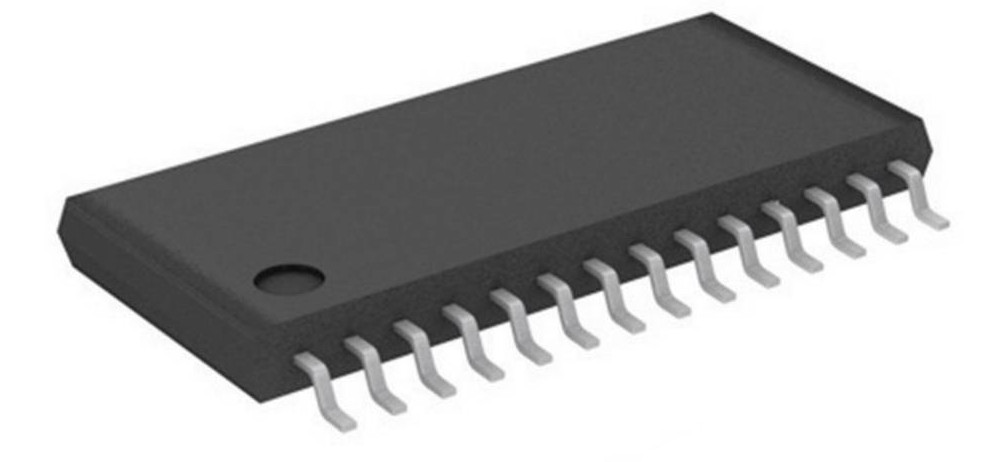
\includegraphics[scale=0.15]{Imagenes/HTSSOP.jpg}
    \caption{Sensor de tensión, corriente y potencia, modelo LM5056A de Texas Instruments, en su encapsulado tipo HTSSOP-28.}
    \label{encapsulado_LM5056}
\end{figure}

Además de lo ya mencionado, el LM5056A tiene un pin al que se puede conectar un circuito que permite la medición de temperatura mediante la utilización de un transistor NPN modelo MMBT3904 conectado al pin DIODE, y medición de una tensión auxiliar de bajo valor mediante el pin VAUX.\\

En la figura \ref{conexion_LM5056A}, se puede ver el esquema circuital del LM5056A dentro de la plataforma de evaluación. Los pines de medición principales son OUT, SENSE, VIN\_K y VIN. Al pin OUT se conecta la tensión de medición secundaria, que en nuestro caso es la tensión de carga $v_o$ fija de \SI[]{75}[]{\volt}. Luego, entre VIN\_K y SENSE se conecta la resistencia shunt $R_{shunt}$ para la medición de la corriente $i_{FC}$ de máximo de \SI[]{10.5}[]{\ampere}, con un capacitor $C_{shunt}$ de \textit{bypass} en paralelo a $R_{shunt}$ según indicación del fabricante. Finalmente, el pin VIN se conecta al mismo punto circuital que VIN\_K, para poder medir la tensión de celda $v_{FC}$, variable entre \SI[]{30}[]{\volt} y \SI[]{65}[]{\volt}, con un capacitor de bypass para mejorar rendimiento en situaciones ruidosas, según recomendacion de fabricante.\\

\begin{figure}[h]
    \centering
    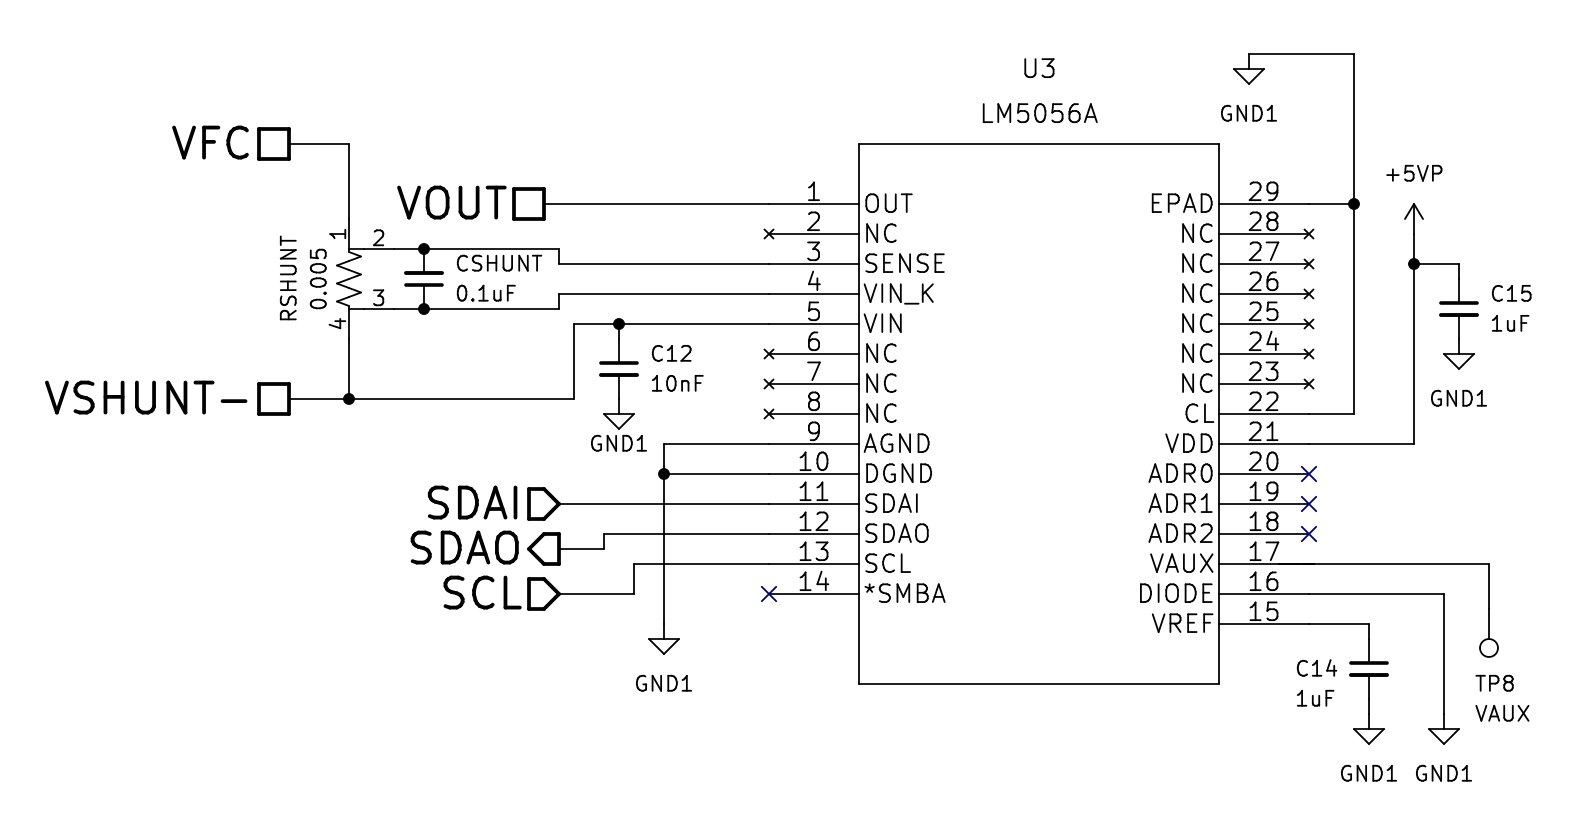
\includegraphics[scale=0.22]{Imagenes/Conexion LM5056A.png}
    \caption{Conexión del sensor LM5056A para medir tensión y corriente de entrada y tensión de salida, según especificaciones del fabricante.}
    \label{conexion_LM5056A}
\end{figure}

Como el dispositivo no tiene aislación incluida, todas sus tierras se conectan al punto común del primario del convertidor, $GND_1$. Luego, el pin CL se utiliza para la selección de rango de medición para la corriente, que puesto a tierra como en la figura, resulta en un fondo de escala de \SI[]{54.4}[]{\milli\volt}. El pin VAUX se deja abierto en caso de ser necesario la medición de una tensión auxiliar, DIODE se deja conectado a masa ya que no se necesita una medición de temperatura. Según el fabricante, al pin VREF se debe conectar un capacitor de bypass desde este pin a $GND_1$. La alimentación del LM5056A, conectado al pin VDD, es de \SI[]{5}[]{\volt}, con un capacitor de bypass en derivación entre alimentación y tierra.\\

Finalmente, para calcular el valor que debe tener el resistor shunt $R_{shunt}$ se toma en cuenta el valor máximo de corriente a medir $i_{FC}$ con algún margen de seguridad, que en nuestro caso es \SI[]{11}[]{\ampere}. Después, utilizando la tensión de fondo de escala de \SI[]{54.4}[]{\milli\volt} elegida para la medición de corriente, se puede obtener el valor de $R_{shunt}$ realizando el cociente entre tensión y corriente, que resulta en un valor de shunt de \SI[]{5}[]{\milli\ohm}.

\begin{equation}\label{calculo_shunt}
    \boxed{\highlight{
    R_{shunt} = \frac{I_{in(FSR)}}{i_{FC(max)}} = \frac{\SI{54.4}{\milli\volt}}{\SI{11}{\ampere}} \approx \SI[]{5}[]{\milli\ohm}
    }}
\end{equation}

\subsubsection{Etapa de Acondicionamiento}

Una vez seleccionados los sensores, muchas veces es necesario agregar a la salida de los mismos un circuito de acondicionamiento, cuyo objetivo es adecuar los niveles de tensión y/o corriente que provee la salida del sensor a los niveles que son requeridos en la entrada de la siguiente etapa. En nuestro caso, esta etapa siguiente es el sistema de control de la plataforma, cuyo diseño se va a profundizar más adelante.\\

Para el sensor LM5056A de la figura \ref{conexion_LM5056A} no es necesario implementar ninguna etapa de acondicionamiento, ya que el mismo transmite sus datos a través de su módulo de comunicación sincrónica $I^2C$, actuando como esclavo y el controlador como maestro. Esta dinámica se explica en detalle en la siguiente sección.\\

\paragraph{Acondicionamiento de $\mathbf{i_o}$}

El sensor de corriente de salida TMCS1100A4 de la figura \ref{conexion_TMCS1100} tiene una salida de tensión analógica, variable linealmente entre \SI[]{0}[]{\volt} y \SI[]{1.8}[]{\volt} para corriente $i_o$ desde nula hasta \SI[]{4.5}[]{\ampere}. Esta señal debe ingresar al conversor analógico-digital de \num{12} bits y \num{4096} niveles del DSC, que toma tensiones de entrada desde \SI[]{0}[]{\volt} hasta \SI[]{3}[]{\volt}.\\

Entonces, como tanto la salida del sensor y la entrada de ADC tienen su origen en tensión nula y solo difieren en la máxima tensión que aceptan, se debe diseñar un circuito de acondicionamiento con una {\Medium ganancia positiva} que lleve los \SI[]{1.8}[]{\volt} del sensor al fondo de escala del ADC, de manera de aprovechar la resolución completa del conversor. Entonces, la ganancia $G_{cc}$ que debemos obtener del circuito se puede obtener con el cociente de las tensiones máximas.

\begin{equation}\label{ganancia_acond}
    G_{cc} = \frac{V_{max(ADC)}}{V_{max(Sensor)}} = \frac{\SI{3}{\volt}}{\SI{1.8}{\volt}} \approx 1.67
\end{equation}

Y como ambas escalas comienzan en cero, no es necesario que el circuito tenga ningún tipo de tensión de offset. Además, la salida del sensor y entrada al ADC del controlador son señales {\Medium \textit{single-ended}} (es decir que solo tiene un conductor para la señal y otro para la tensión de referencia de tierra), por lo que solo es relevante la amplificación single-ended del circuito.\\

Para este propósito, se eligió un {\Medium amplificador diferencial} basado en un amplificador operacional, con una red de resistencias y capacitores que definen su ganancia $A_d$ y ancho de banda $BW$, que observa en la figura \ref{circuito_acond}. Este circuito, además de proveer la adaptación de niveles, actúa como un filtro pasabajos que le da al sistema una mayor inmunidad al ruido.\\

\begin{figure}[h]
    \centering
    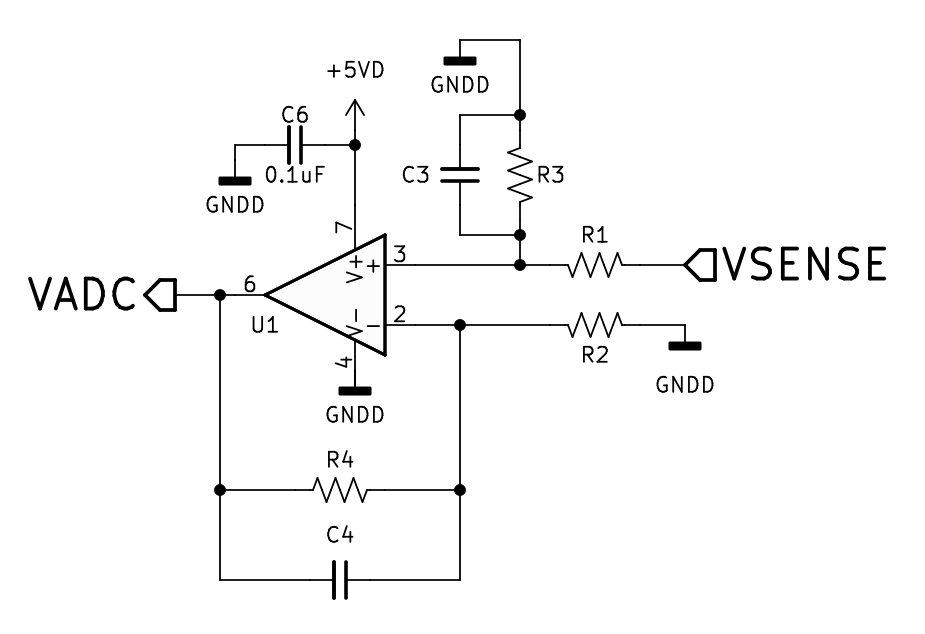
\includegraphics[scale=1.2]{Imagenes/Acondicionamiento.png}
    \caption{Circuito del amplificador diferencial de acondicionamiento, utilizando un amplificador operacional.}
    \label{circuito_acond}
\end{figure}

Como el amplificador es diferencial pero la tensión a la entrada es single-ended ,y no se busca un amplificador inversor, se conecta la tensión de salida del sensor al pin positivo de entrada del operacional, con el pin negativo conectado a tierra. En este amplificador, se deben cumplir un par de condiciones, particularmente, las resistencias $R_1$ y $R_2$ deben ser iguales, al igual que las impedancias $Z_3$ y $Z_4$, que resultan del paralelo de las resistencias y las impedancias de los capacitores $C_3$ y $C_4$ a la frecuencia $f_s$ de interés de \SI[]{20}[]{\kilo\hertz}.\\

Con estas condiciones, y asumiendo las características de un amplificador operacional ideal (tensiones $v_+$ y $v_-$ idénticas, y corrientes $i_+$ e $i_-$ nulas), se obtienen las siguientes dos expresiones para la ganancia y el ancho de banda del circuito.\textsuperscript{\cite{Caravelli-Irusta}\cite{DifferenceAmps}}\\

\begin{equation}\label{ec_gcc}
    G_{cc} = \frac{Z_3}{R_1} = \frac{Z_4}{R_2}
\end{equation}

\begin{equation}\label{ec_bw}
    BW = \frac{1}{2\pi R_3C_3} = \frac{1}{2\pi R_4C_4}
\end{equation}

Entonces, si tomamos como requerimientos la ganancia $G_{cc}$ de \num{1.67} de la ecuación \ref{ganancia_acond} y un ancho de banda $BW$ (frecuencia de \SI[]{-3}[]{\deci\bel}) de \SI[]{100}[]{\kilo\hertz} mucho mayor a la frecuencia de conmutación del convertidor, y elegimos (arbitrariamente) resistencias $R_1$ y $R_2$ de \SI[]{16.5}[]{\kilo\ohm}, podemos despejar entonces la impedancia $Z_3$ de la ecuación \ref{ec_gcc}.

\begin{equation}
    Z_3 = Z_4 = G_{cc}R_1 = \SI{27.55}{\kilo\ohm}
\end{equation}

Con este valor y los requerimientos más arriba, tenemos que calcular los valores de ambos componentes del paralelo de $Z_3$ (o $Z_4$), $R_3$ y $C_3$ (o $R_4$ y $C_4$). Con este objetivo, planteamos la ecuación este paralelo.

\begin{equation}
    Z_3 = \frac{R_3\cdot X_{C3}}{R_3+X_{C3}} = \SI{27.55}{\kilo\ohm}
\end{equation}

Donde $X_{C3}$ es la impedancia capacitiva del paralelo, definido como el inverso del producto de la frecuencia angular de interés por la capacidad del capacitor $C_3$. Reemplazando por esta expresión, obtenemos la siguiente ecuación.

\begin{equation}\label{eq_z3}
        Z_3 = \frac{R_3}{2\pi fC_3R_3 + 1} = \SI[]{27.55}[]{\kilo\ohm}
\end{equation}

Con esta ecuación y la ecuación \ref{ec_bw} del ancho de banda de la topología, podemos conformar un sistema de ecuaciones de dos variables y dos ecuaciones no lineales.

\begin{equation}\label{sist_eq}
    \begin{aligned}
        \frac{R_3}{2\pi fC_3R_3 + 1} &= \SI[]{27.55}[]{\kilo\ohm}\\
        \frac{1}{2\pi R_3C_3}        &= \SI[]{100}[]{\kilo\hertz}
    \end{aligned}
\end{equation}

Entonces, si despejamos $R_3$ y $C_3$ de este sistema de ecuaciones, obtenemos los siguientes valores para los mismos (recordar que $R_4$ y $C_4$ deben ser idénticos).

\begin{equation*}
    \begin{aligned}
        R_3 = R_4 &= \SI[]{33.06}[]{\kilo\ohm}\\
        C_3 = C_4 &= \SI[]{48.1}[]{\pico\farad}
    \end{aligned}
\end{equation*}

Ahora solo falta redondear estos parámetros a los valores comerciales más cercanos para cada uno de los componentes, que se observan en la siguiente tabla.\\

\setlength{\tabcolsep}{8pt}
\renewcommand{\arraystretch}{1.5}
\begin{table}[H]
\begin{center}
    \begin{tabular}{rrrrrr}
    $\mathbf{R_1}$ [\unit{\kilo\ohm}] & $\mathbf{R_2}$ [\unit{\kilo\ohm}] & $\mathbf{R_3}$ [\unit{\kilo\ohm}] & $\mathbf{R_4}$ [\unit{\kilo\ohm}] & $\mathbf{C_3}$ [\unit{\pico\farad}] & $\mathbf{C_4}$ [\unit{\pico\farad}]\\
    \hline
    \num{16.5} & \num{16.5} & \num{33} & \num{33} & \num{47} & \num{47}
    \end{tabular}
    \caption{Valores comerciales de todas las resistencias y capacitores del circuito de acondicionamiento.}
    \label{tabla:componentes_acond}
\end{center}
\end{table}

Si usamos estos valores finales para calcular las especificaciones de las ecuaciones de ganancia y ancho de banda, se obtienen los siguientes valores:

\begin{equation*}
    \boxed{\highlight{
    \begin{aligned}
        G_{cc} &= \num{1.673}\\
        BW &= \SI[]{102.6}[]{\kilo\hertz}
    \end{aligned}
    }}
\end{equation*}

\paragraph{Selección del Amplificador Operacional}

Con el circuito de acondicionamiento diseñado y dimensionado ahora solo queda la elección de un amplificador operacional para utilizar en el circuito, que cumpla los siguientes requerimientos.\\

\begin{itemize}
    \item Debe ser un amplificador \textit{rail-to-rail}, es decir que sea capaz de amplificar hasta la tensión de alimentación.
    \item Ancho de banda mucho mayor a \SI[]{100}[]{\kilo\hertz}.
    \item Encapsulado pequeño de montaje superficial.\\
\end{itemize}

Buscando en los dispositivos disponibles en el laboratorio, se eligió utilizar el modelo {\Medium OPA365} de Texas Instruments, un amplificador operacional rail-to-rail de encapsulado SMD tipo SOIC-8, idéntico al del sesnor TMCS1100A4 de la figura \ref{encapsulado_hall}. Se marcaron algunas de sus especificaciones más importantes en la siguiente tabla.\\

\setlength{\tabcolsep}{7pt}
\renewcommand{\arraystretch}{1.5}
\begin{table}[H]
\begin{center}
    \begin{tabular}{llrrrr}
    {\SemiBold Fabricante} & {\SemiBold Modelo} & $\mathbf{V_{in(max)}}$ [\unit{\volt}] & $\mathbf{V_{DD(max)}}$ [\unit{\volt}] & $\mathbf{A_{OL}}$ [\unit{\deci\bel}] & $\mathbf{GBW}$ [\unit{\mega\hertz}]\\
    \hline
    Texas Instruments & OPA365 & $V_{DD}$ + \num{0.5} & \num{5.5} &  \num{120} & \num{50}
    \end{tabular}
    \caption{Especificaciones del amplificador operacional modelo OPA365 de Texas Instruments.\textsuperscript{\cite{OPA365}}}
    \label{tabla:OPA365}
\end{center}
\end{table}

Al ubicarse el circuito de acondicionamiento a continuación de la salida del sensor de efecto Hall TMCS1100A4 (que provee su propia aislación galvánica), las conexiones a tierra de todas las partes deben ser conectadas a la tierra digital o de señal $GND_D$.\\

\subsubsection{Etapa de Transmisión}

{\Bold\scshape Falta completar esta sección.}\\

\lipsum[2]\\

\begin{figure}[h]
    \centering
    
\includegraphics[scale=1]{Imagenes/Logo I2C.pdf}
    \caption{Logotipo del protocolo de bus comunicación serie I\textsuperscript{2}C.}
    \label{logo_I2C}
\end{figure}

\lipsum[3]\\

\newpage

\subsection{Etapa de Aislación de Señal}

Ahora se debe implementar un circuito auxiliar que provea una aislación galvánica entre los componentes que se sitúan del lado de potencia de la plataforma (como los transistores, diodos, circuito driver, etc.), y los componentes de la parte digital del sistema (como el controlador digital de señales, el circuito de acondicionamiento, etc.).\\

Existen tres partes principales de la plataforma, donde se pasa de la parte digital a la de potencia, donde se requiere algún tipo de aislación:\\

\begin{enumerate}
    \item Entre las salidas PWM del controlador y las entradas de comando de los drivers 2ED21834-S06J de la figura \ref{circuito_driver}.
    \item Para las líneas del bus I\textsuperscript{2}C que comunican al sensor LM5056A de la figura \ref{conexion_LM5056A} (lado de potencia) con el módulo I\textsuperscript{2}C del controlador.
    \item Para la medición de corriente de salida mediante el sensor de efecto Hall TMCS1100A4 de la figura \ref{conexion_TMCS1100}.
    \item Para generar fuentes de alimentación aisladas para los circuitos del lado digital.\\
\end{enumerate}

En este capítulo vamos a tratar las soluciones de aislación para los primeros dos casos. En el tercer caso, el TMCS1100A4, al ser un dispositivo que funciona por medio del efecto Hall, ya tiene aislación incluida en su diseño, por lo que la salida del mismo ya se encuentra aislada del convertidor. Para el cuarto ítem, esto se va a tratar propiamente y en profundidad en la sección de este capítulo dedicada a los circuitos de alimentación de la plataforma.\\

\subsubsection{Tecnologías de Aislación de Señal}

{\Bold\scshape Falta completar esta sección.}\\

\lipsum[1]\\

\subsubsection{Aislación de los Drivers}

Cómo los drivers están conectados directamente a terminales de los transistores de potencia del convertidor, estos se encuentran dentro de la etapa de potencia de la plataforma. Sin embargo, las señales PWM que definen el tiempo y secuencia de conmutación de los transistores provienen del módulo PWM del controlador digital, todo dentro del área digital de la plataforma. Entonces, previo a las entradas de señal de los 2ED21834-S06J se debe interponer algun circuito de aislación de señal, para mantener la separación entre potencia y señal.\\

\lipsum[2]\\

\subsubsection{Aislación I\textsuperscript{2}C}

\lipsum[2]\\



\newpage

\subsection{Sistema de Control}

{\Large\Bold\scshape Falta completar esta sección.}\\

\lipsum[1]\\

\lipsum[2]\\

\newpage

\subsection{Circuito de Alimentación}

\lipsum[3]\\

\lipsum[4]\\

\newpage

\subsection{Resumen}

\lipsum[1]\\

\lipsum[2]\\

\newpage